\documentclass[
  shownotes,
  xcolor={svgnames},
  hyperref={colorlinks,citecolor=DarkBlue,linkcolor=DarkRed,urlcolor=DarkBlue}
   , aspectratio=169]{beamer}

\usepackage{animate}
\usepackage{amsmath}
\usepackage{amsfonts}
\usepackage{amssymb}
\usepackage{pifont}
\usepackage{mathpazo}
%\usepackage{xcolor}
\usepackage{multimedia}
\usepackage{fancybox}
\usepackage[para]{threeparttable}
\usepackage{multirow}
\setcounter{MaxMatrixCols}{30}
\usepackage{subcaption}
\usepackage{graphicx}
\usepackage{lscape}
\usepackage[compatibility=false,font=small]{caption}
\usepackage{booktabs}
\usepackage{ragged2e}
\usepackage{chronosys}
\usepackage{appendixnumberbeamer}
\usepackage{animate}
\setbeamertemplate{caption}[numbered]
\usepackage{color}
%\usepackage{times}
\usepackage{tikz}
\usepackage{comment} %to comment
%% BibTeX settings
\usepackage{natbib}
\bibliographystyle{apalike}
\bibpunct{(}{)}{,}{a}{,}{,}
\setbeamertemplate{bibliography item}{[\theenumiv]}

% Defines columns for bespoke tables
\usepackage{array}
\newcolumntype{L}[1]{>{\raggedright\let\newline\\\arraybackslash\hspace{0pt}}m{#1}}
\newcolumntype{C}[1]{>{\centering\let\newline\\\arraybackslash\hspace{0pt}}m{#1}}
\newcolumntype{R}[1]{>{\raggedleft\let\newline\\\arraybackslash\hspace{0pt}}m{#1}}


\usepackage{xfrac}


\usepackage{multicol}
\setlength{\columnsep}{0.5cm}

% Theme and colors
\usetheme{Boadilla}

% I use steel blue and a custom color palette. This defines it.
\definecolor{andesred}{HTML}{af2433}

% Other options
\providecommand{\U}[1]{\protect\rule{.1in}{.1in}}
\usefonttheme{serif}
\setbeamertemplate{itemize items}[default]
\setbeamertemplate{enumerate items}[square]
\setbeamertemplate{section in toc}[circle]

\makeatletter

\definecolor{mybackground}{HTML}{82CAFA}
\definecolor{myforeground}{HTML}{0000A0}

\setbeamercolor{normal text}{fg=black,bg=white}
\setbeamercolor{alerted text}{fg=red}
\setbeamercolor{example text}{fg=black}

\setbeamercolor{background canvas}{fg=myforeground, bg=white}
\setbeamercolor{background}{fg=myforeground, bg=mybackground}

\setbeamercolor{palette primary}{fg=black, bg=gray!30!white}
\setbeamercolor{palette secondary}{fg=black, bg=gray!20!white}
\setbeamercolor{palette tertiary}{fg=white, bg=andesred}

\setbeamercolor{frametitle}{fg=andesred}
\setbeamercolor{title}{fg=andesred}
\setbeamercolor{block title}{fg=andesred}
\setbeamercolor{itemize item}{fg=andesred}
\setbeamercolor{itemize subitem}{fg=andesred}
\setbeamercolor{itemize subsubitem}{fg=andesred}
\setbeamercolor{enumerate item}{fg=andesred}
\setbeamercolor{item projected}{bg=gray!30!white,fg=andesred}
\setbeamercolor{enumerate subitem}{fg=andesred}
\setbeamercolor{section number projected}{bg=gray!30!white,fg=andesred}
\setbeamercolor{section in toc}{fg=andesred}
\setbeamercolor{caption name}{fg=andesred}
\setbeamercolor{button}{bg=gray!30!white,fg=andesred}


\usepackage{fancyvrb}
\newcommand{\VerbBar}{|}
\newcommand{\VERB}{\Verb[commandchars=\\\{\}]}
\DefineVerbatimEnvironment{Highlighting}{Verbatim}{commandchars=\\\{\}}
% Add ',fontsize=\small' for more characters per line
\usepackage{framed}
\definecolor{shadecolor}{RGB}{248,248,248}
\newenvironment{Shaded}{\begin{snugshade}}{\end{snugshade}}
\newcommand{\AlertTok}[1]{\textcolor[rgb]{0.94,0.16,0.16}{#1}}
\newcommand{\AnnotationTok}[1]{\textcolor[rgb]{0.56,0.35,0.01}{\textbf{\textit{#1}}}}
\newcommand{\AttributeTok}[1]{\textcolor[rgb]{0.77,0.63,0.00}{#1}}
\newcommand{\BaseNTok}[1]{\textcolor[rgb]{0.00,0.00,0.81}{#1}}
\newcommand{\BuiltInTok}[1]{#1}
\newcommand{\CharTok}[1]{\textcolor[rgb]{0.31,0.60,0.02}{#1}}
\newcommand{\CommentTok}[1]{\textcolor[rgb]{0.56,0.35,0.01}{\textit{#1}}}
\newcommand{\CommentVarTok}[1]{\textcolor[rgb]{0.56,0.35,0.01}{\textbf{\textit{#1}}}}
\newcommand{\ConstantTok}[1]{\textcolor[rgb]{0.00,0.00,0.00}{#1}}
\newcommand{\ControlFlowTok}[1]{\textcolor[rgb]{0.13,0.29,0.53}{\textbf{#1}}}
\newcommand{\DataTypeTok}[1]{\textcolor[rgb]{0.13,0.29,0.53}{#1}}
\newcommand{\DecValTok}[1]{\textcolor[rgb]{0.00,0.00,0.81}{#1}}
\newcommand{\DocumentationTok}[1]{\textcolor[rgb]{0.56,0.35,0.01}{\textbf{\textit{#1}}}}
\newcommand{\ErrorTok}[1]{\textcolor[rgb]{0.64,0.00,0.00}{\textbf{#1}}}
\newcommand{\ExtensionTok}[1]{#1}
\newcommand{\FloatTok}[1]{\textcolor[rgb]{0.00,0.00,0.81}{#1}}
\newcommand{\FunctionTok}[1]{\textcolor[rgb]{0.00,0.00,0.00}{#1}}
\newcommand{\ImportTok}[1]{#1}
\newcommand{\InformationTok}[1]{\textcolor[rgb]{0.56,0.35,0.01}{\textbf{\textit{#1}}}}
\newcommand{\KeywordTok}[1]{\textcolor[rgb]{0.13,0.29,0.53}{\textbf{#1}}}
\newcommand{\NormalTok}[1]{#1}
\newcommand{\OperatorTok}[1]{\textcolor[rgb]{0.81,0.36,0.00}{\textbf{#1}}}
\newcommand{\OtherTok}[1]{\textcolor[rgb]{0.56,0.35,0.01}{#1}}
\newcommand{\PreprocessorTok}[1]{\textcolor[rgb]{0.56,0.35,0.01}{\textit{#1}}}
\newcommand{\RegionMarkerTok}[1]{#1}
\newcommand{\SpecialCharTok}[1]{\textcolor[rgb]{0.00,0.00,0.00}{#1}}
\newcommand{\SpecialStringTok}[1]{\textcolor[rgb]{0.31,0.60,0.02}{#1}}
\newcommand{\StringTok}[1]{\textcolor[rgb]{0.31,0.60,0.02}{#1}}
\newcommand{\VariableTok}[1]{\textcolor[rgb]{0.00,0.00,0.00}{#1}}
\newcommand{\VerbatimStringTok}[1]{\textcolor[rgb]{0.31,0.60,0.02}{#1}}
\newcommand{\WarningTok}[1]{\textcolor[rgb]{0.56,0.35,0.01}{\textbf{\textit{#1}}}}
\usepackage{graphicx}
\makeatletter

\usepackage{tikz}
% Tikz settings optimized for causal graphs.
\usetikzlibrary{shapes,decorations,arrows,calc,arrows.meta,fit,positioning}
\tikzset{
    -Latex,auto,node distance =1 cm and 1 cm,semithick,
    state/.style ={ellipse, draw, minimum width = 0.7 cm},
    point/.style = {circle, draw, inner sep=0.04cm,fill,node contents={}},
    bidirected/.style={Latex-Latex,dashed},
    el/.style = {inner sep=2pt, align=left, sloped}
}


\makeatother






%%%%%%%%%%%%%%% BEGINS DOCUMENT %%%%%%%%%%%%%%%%%%

\begin{document}

\title[Lecture 11]{Lecture 11: \\ Intro to Spatial Data}
\subtitle{Big Data and Machine Learning for Applied Economics \\ Econ 4676}
\date{\today}

\author[Sarmiento-Barbieri]{Ignacio Sarmiento-Barbieri}
\institute[Uniandes]{Universidad de los Andes}


\begin{frame}[noframenumbering]
\maketitle
\end{frame}

%%%%%%%%%%%%%%%%%%%%%%%%%%%%%%%%%%%


%----------------------------------------------------------------------%
\begin{frame}
\frametitle{Announcement }


\begin{itemize} 
    \item {\bf Problem Set 2 is due next Thursday September 16 at 1:00pm} 
    \medskip
    \item At some point before the class I'll send what points everyone should present. You should be prepared. Your grade will be impacted if you are not ready. 
    \medskip
    \item  I expect good presentations. You are encouraged to consider it as a mini-seminar, just 2-5 minutes using one or two slides
    \medskip
    \item  Attempt to make a concise interpretation of the relevant material, making effective use of supporting numerical and graphical evidence.    
\end{itemize}
\end{frame}

%----------------------------------------------------------------------% 

\begin{frame}
\frametitle{Agenda}

\tableofcontents

\end{frame}




%----------------------------------------------------------------------%
\section{Spatial Data }
\subsection{Motivation }
%----------------------------------------------------------------------%


\begin{frame}[fragile]
\frametitle{Motivation}


\begin{itemize}
  \item In Big Data  volume was only a part of the story 
  \bigskip
  \item Big Data are data of high complexity: anarchic and spontaneous
  \bigskip
  \item They are the by product of an action: pay with credit card, tweet, move from point A to point B, buy a house, etc.
	\bigskip
  \item Now we are going to focus on spatial data
\end{itemize}

\end{frame}


%----------------------------------------------------------------------%
\begin{frame}[fragile]
\frametitle{Motivation}

\begin{figure}[H] \centering
  \centering
  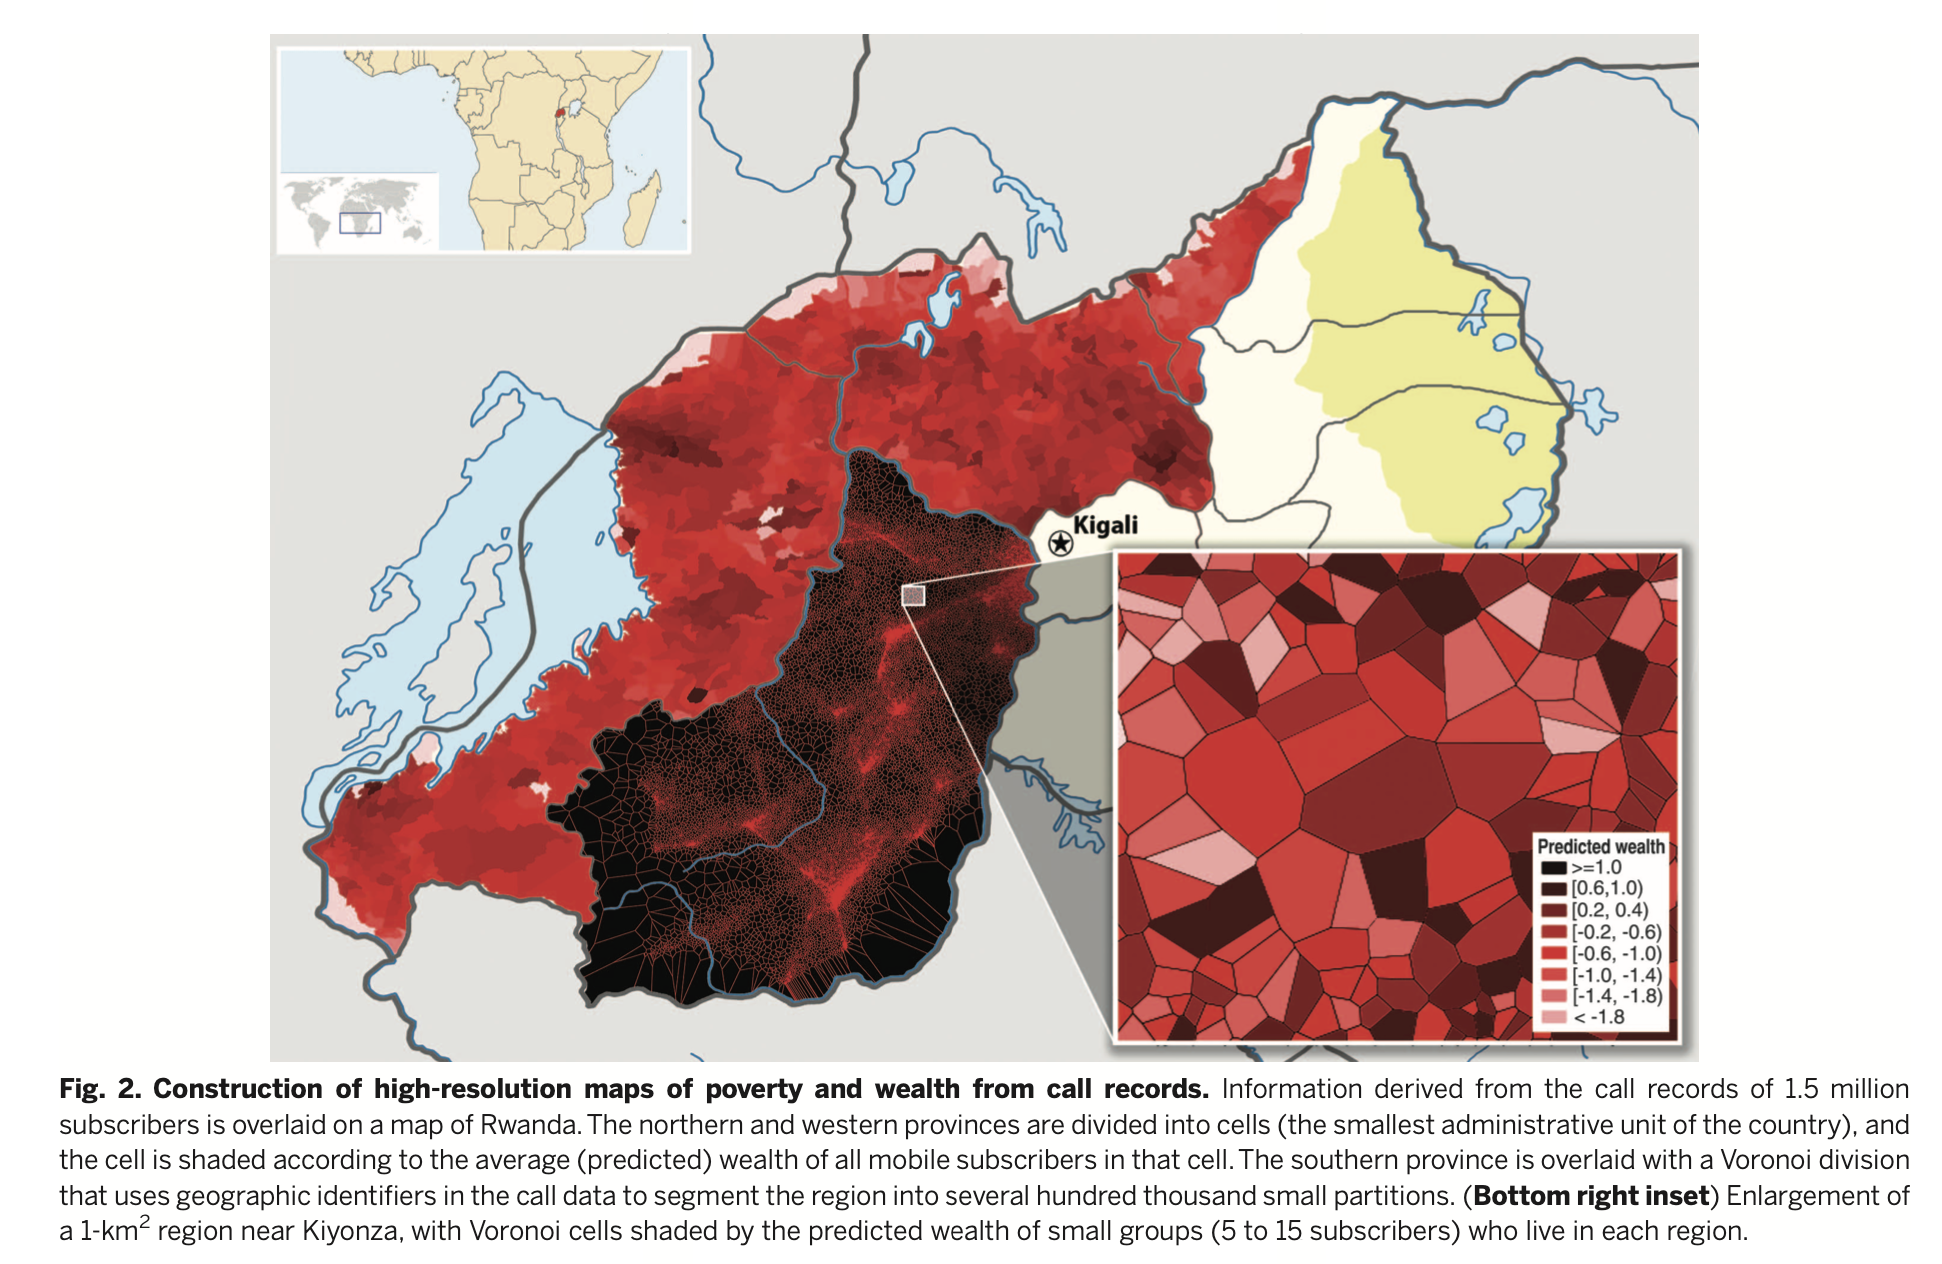
\includegraphics[scale=0.3]{figures/blumenstock_fig2.png}
  \\
  \tiny Blumenstock et al (2015)
\end{figure}

\end{frame}


%----------------------------------------------------------------------%
\begin{frame}[fragile]
\frametitle{Motivation}

\begin{figure}[H] \centering
  \centering
  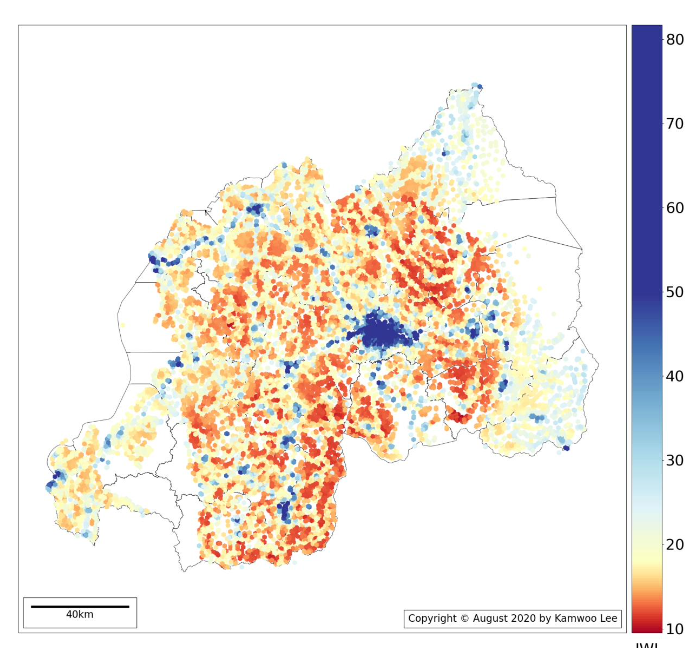
\includegraphics[scale=0.5]{figures/lee_rwanda}
  \\
  \tiny Lee, K., \& Braithwaite, J. (2020)
\end{figure}


\end{frame}

%----------------------------------------------------------------------%
\subsection{Types of Spatial Data}
%----------------------------------------------------------------------%
\begin{frame}[fragile]
\frametitle{Types of Spatial Data}
Spatial data comes in many ``shapes'' and ``sizes'', the most common types of spatial data are:
\medskip
\begin{itemize}
	\item Points are the most basic form of spatial data. Denotes a single point location, such as cities, a GPS reading, or any other discrete object defined in space.
	\medskip
	\item Lines are a set of ordered points, connected by straight line segments
	\medskip
	\item Polygons denote an area, and can be thought as a sequence of connected points, where the first point is the same as the last
	\medskip
	\item Grid (Raster) are a collection of points or rectangular cells, organized in a regular lattice.
\end{itemize}

\end{frame}
%----------------------------------------------------------------------%
\begin{frame}[fragile]
\frametitle{Types of Spatial Data: Points}

\begin{figure}[H] \centering
  
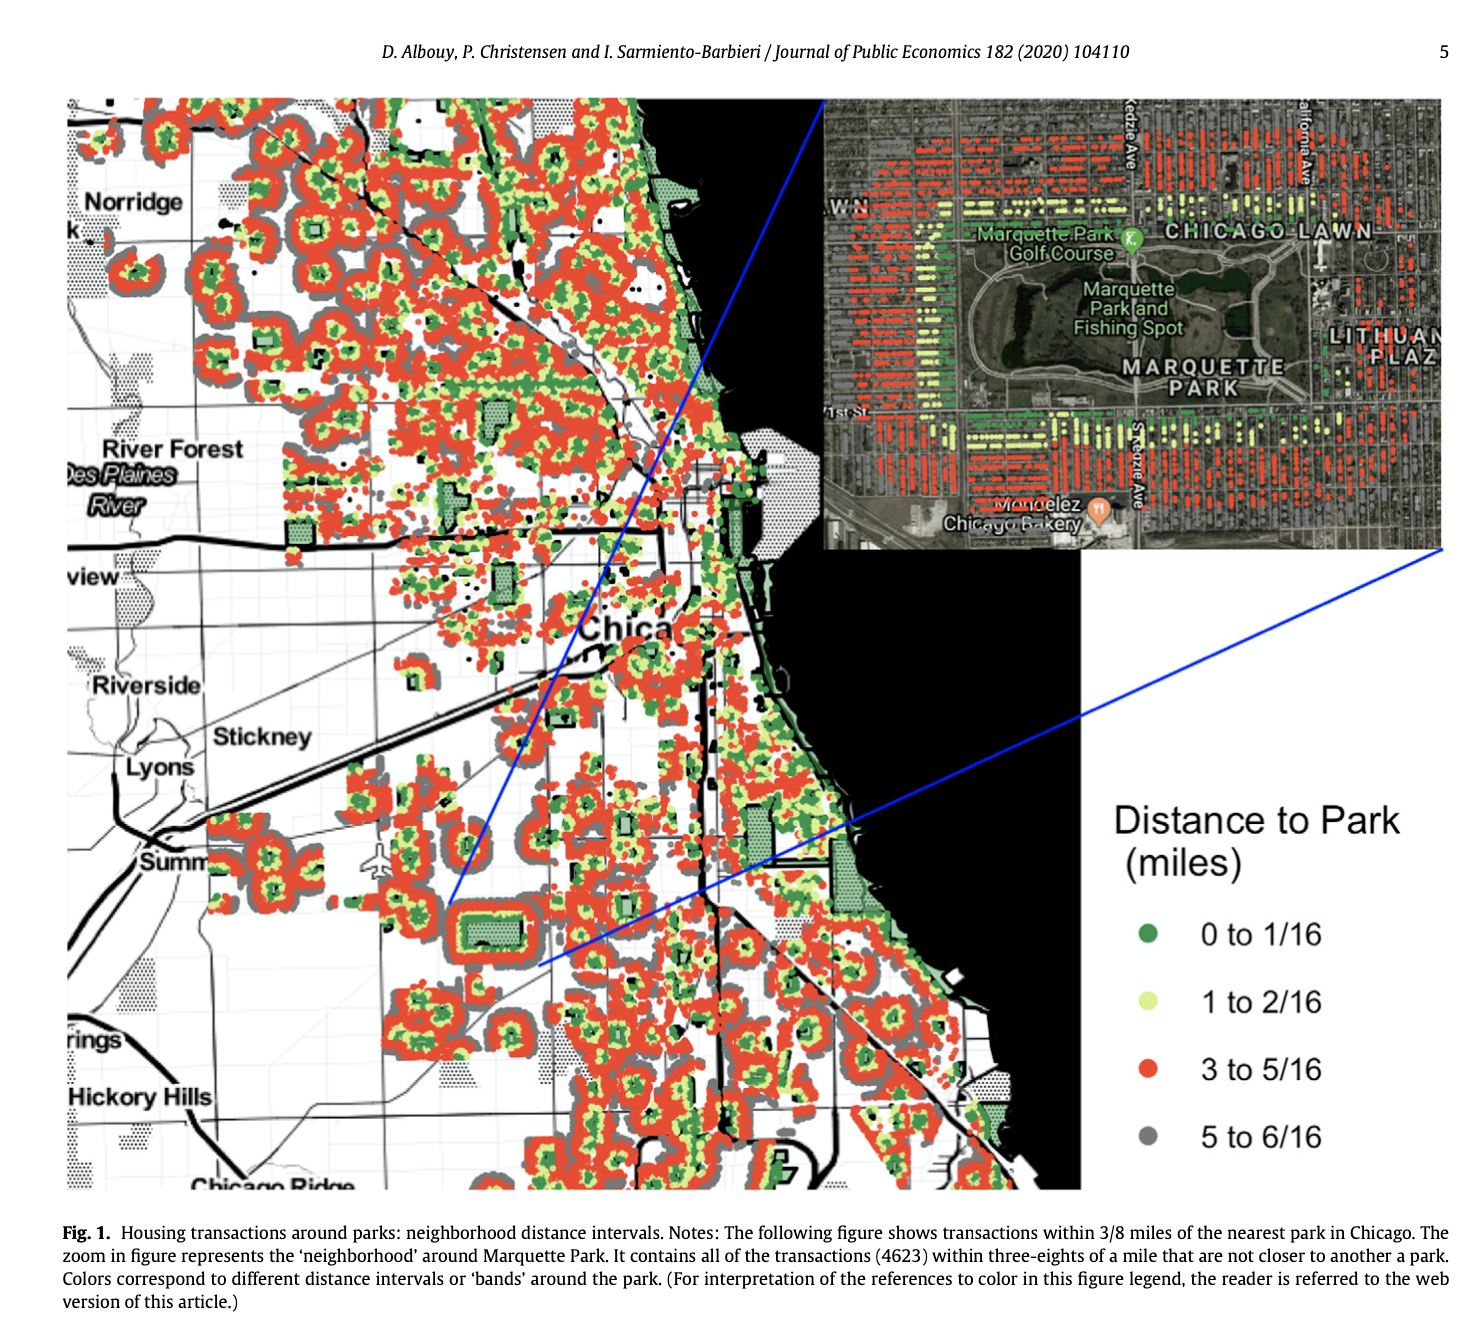
\includegraphics[scale=0.35]{figures/albouy_et_al_fig1.png}
  \\
  \tiny Albouy, Christensen, \& Sarmiento-Barbieri (2020)
\end{figure}


\end{frame}

%----------------------------------------------------------------------%
\begin{frame}[fragile]
\frametitle{Types of Spatial Data: Lines}

\begin{figure}[H] 
  \centering
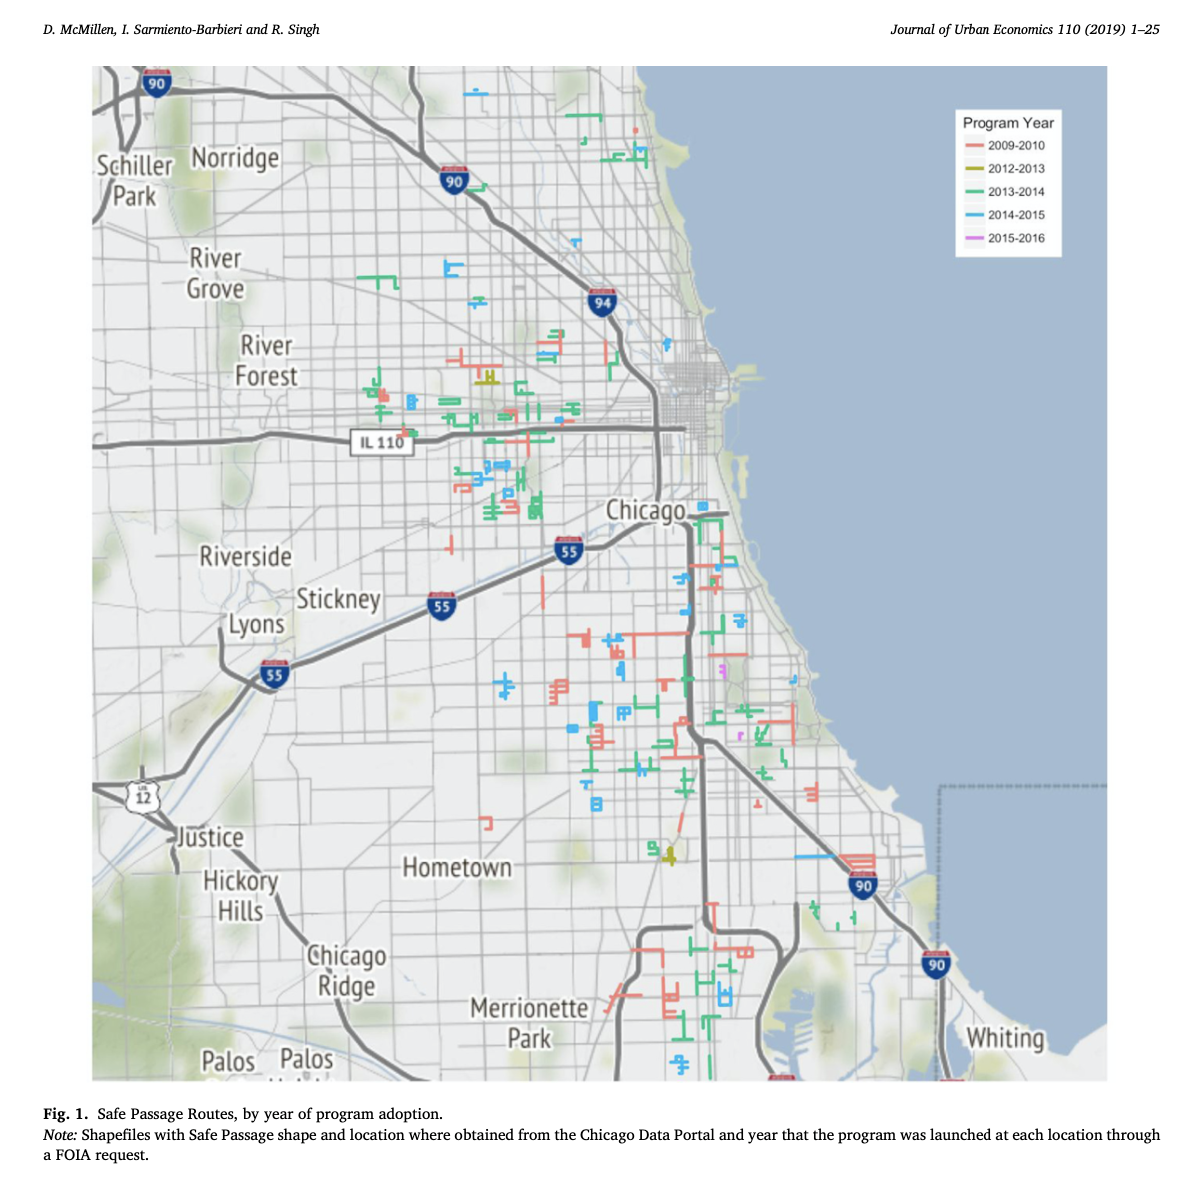
\includegraphics[scale=0.35]{figures/safe_passage.png}
  \\
\tiny McMillen, Sarmiento-Barbieri \& Singh, 2019

\end{figure}

\end{frame}

%----------------------------------------------------------------------%
\begin{frame}[fragile]
\frametitle{Types of Spatial Data: Polygons}

\begin{figure}[H] \centering
  \centering
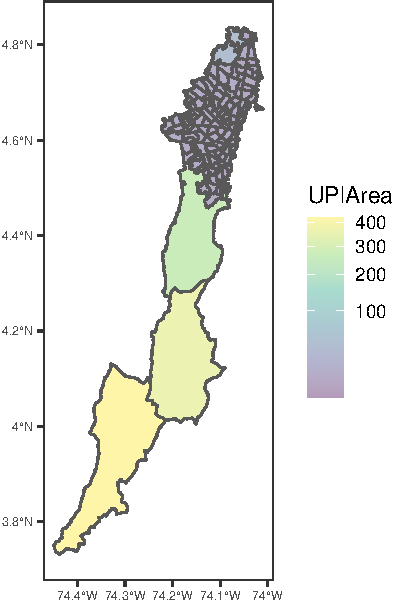
\includegraphics[scale=0.60]{figures/upz.pdf}
  \\
  \tiny Source:\url{https://datosabiertos.bogota.gov.co/dataset/unidad-de-planeamiento-bogota-d-c}
\end{figure}



\end{frame}

%----------------------------------------------------------------------%
\begin{frame}[fragile]
\frametitle{Types of Spatial Data: Combination}

\begin{figure}[H] \centering
  \centering
  
\begin{subfigure}{0.45\linewidth}
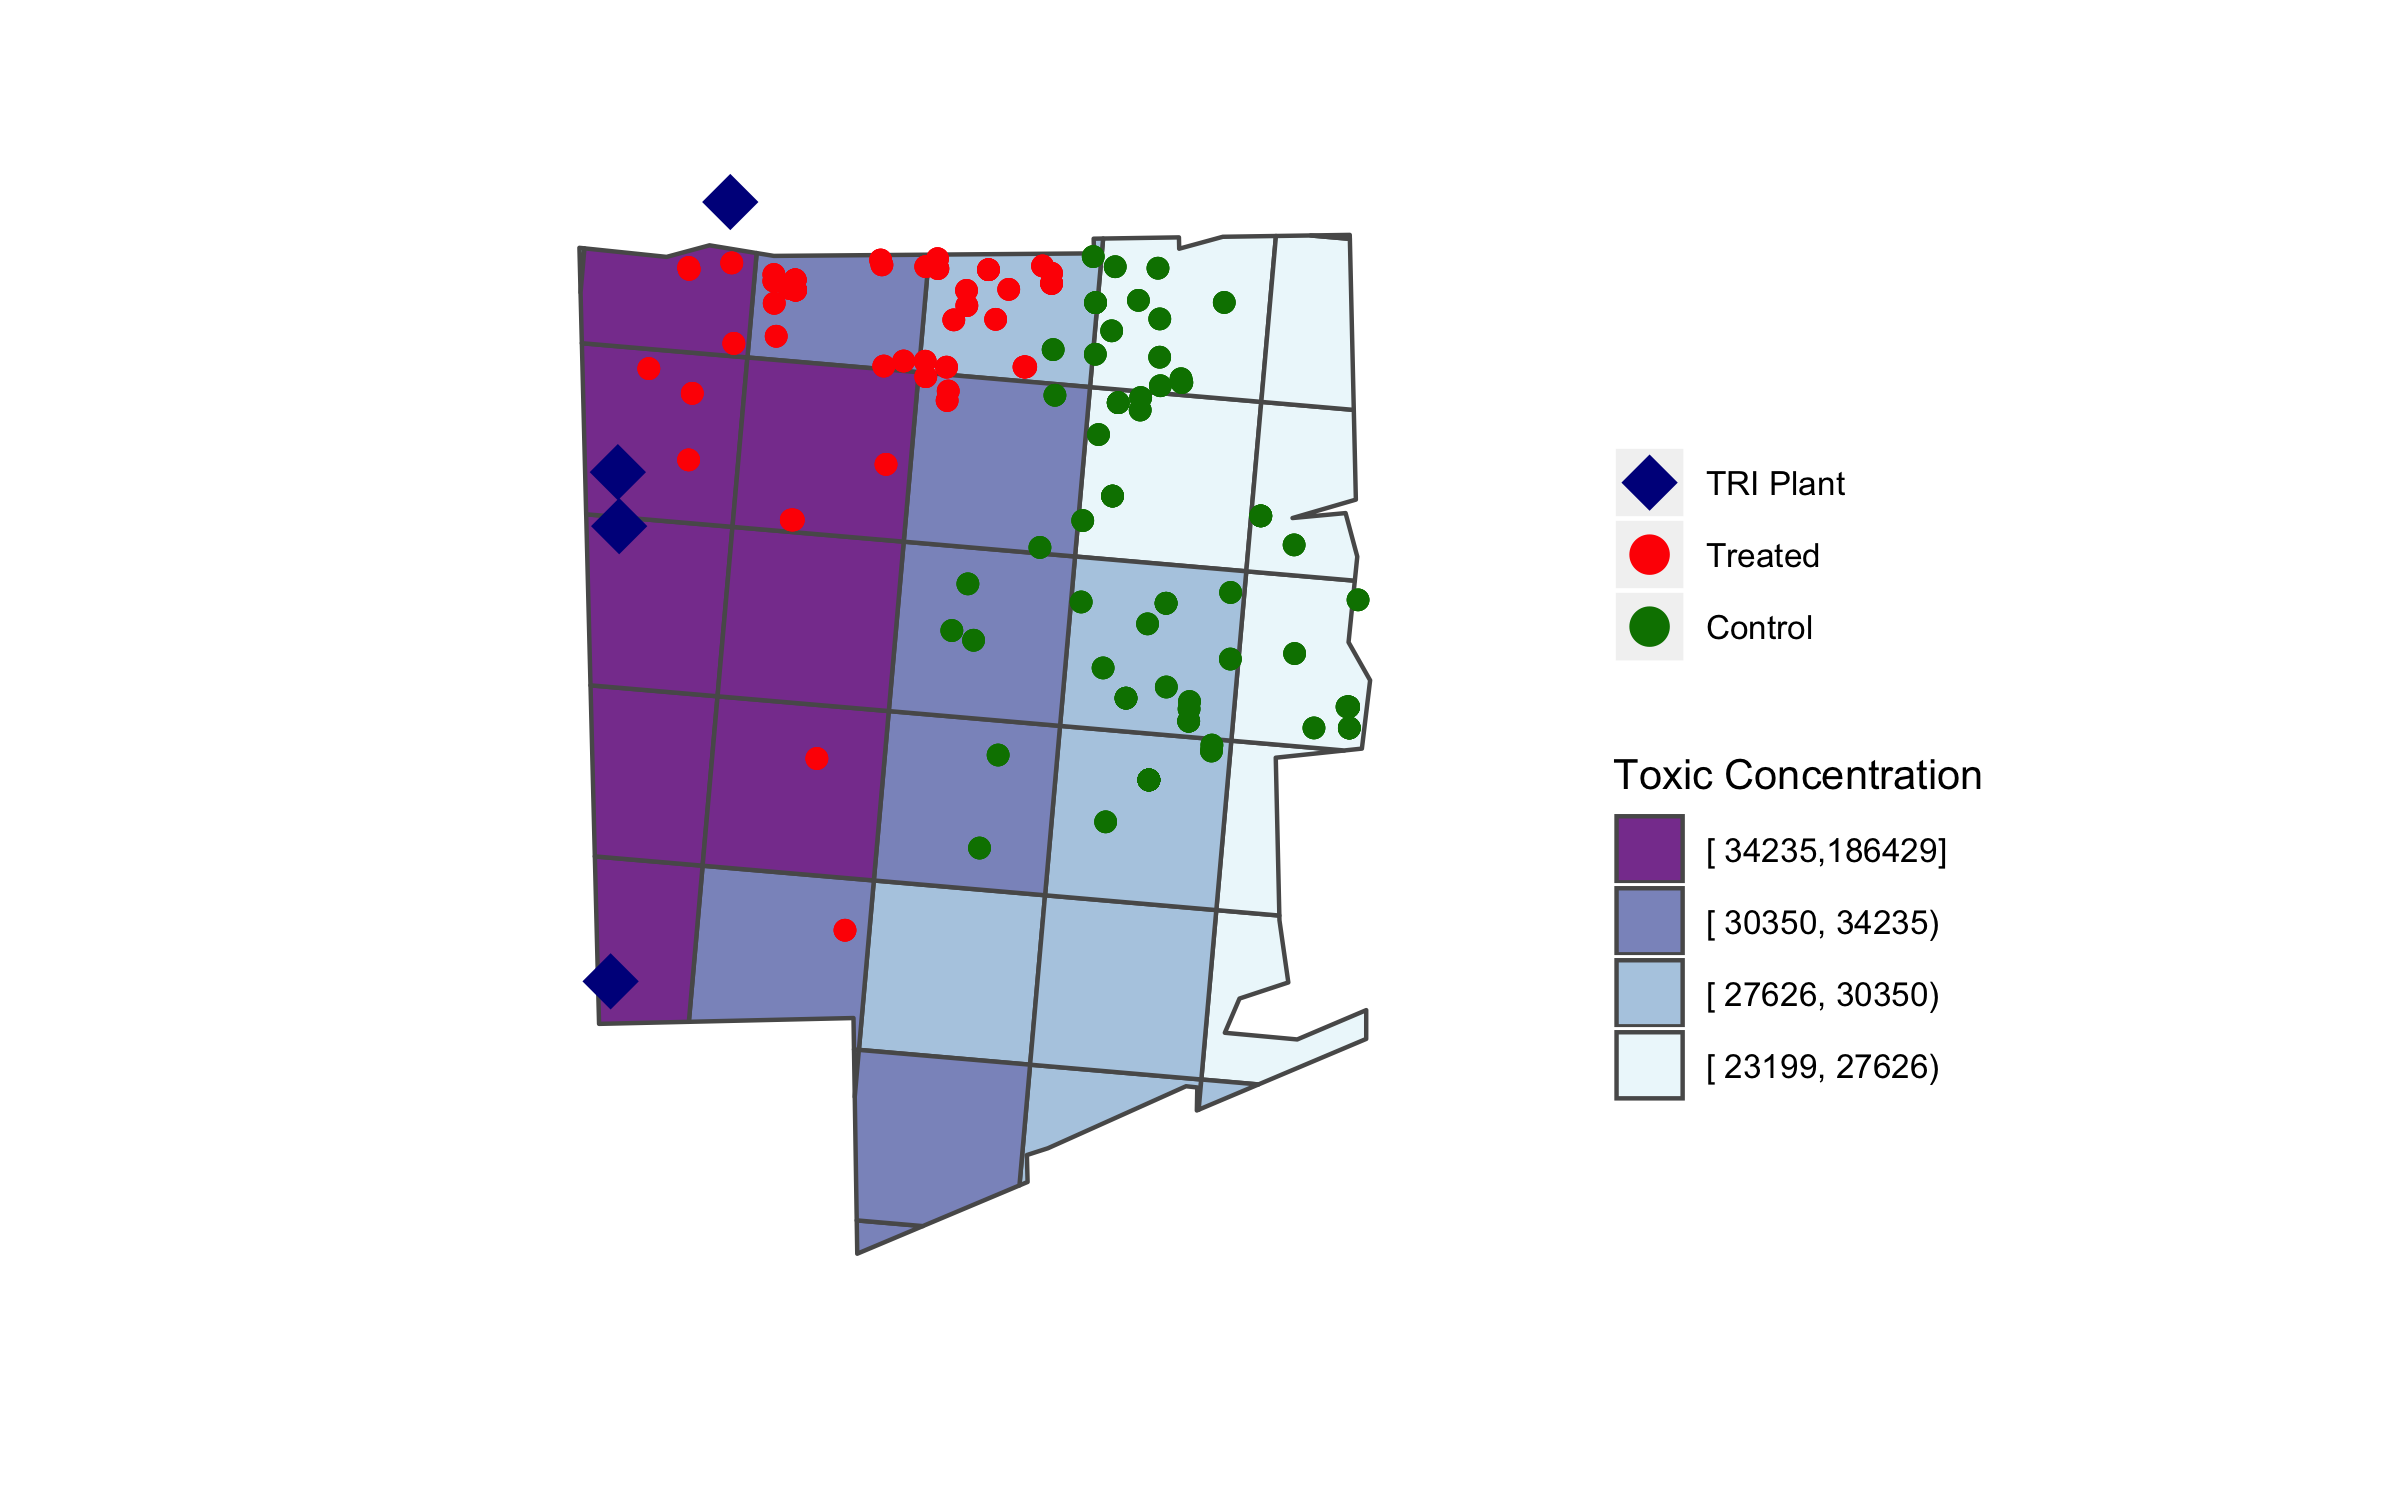
\includegraphics[scale=0.08]{figures/ZIP_A.png}
\end{subfigure}
\begin{subfigure}{0.45\linewidth}
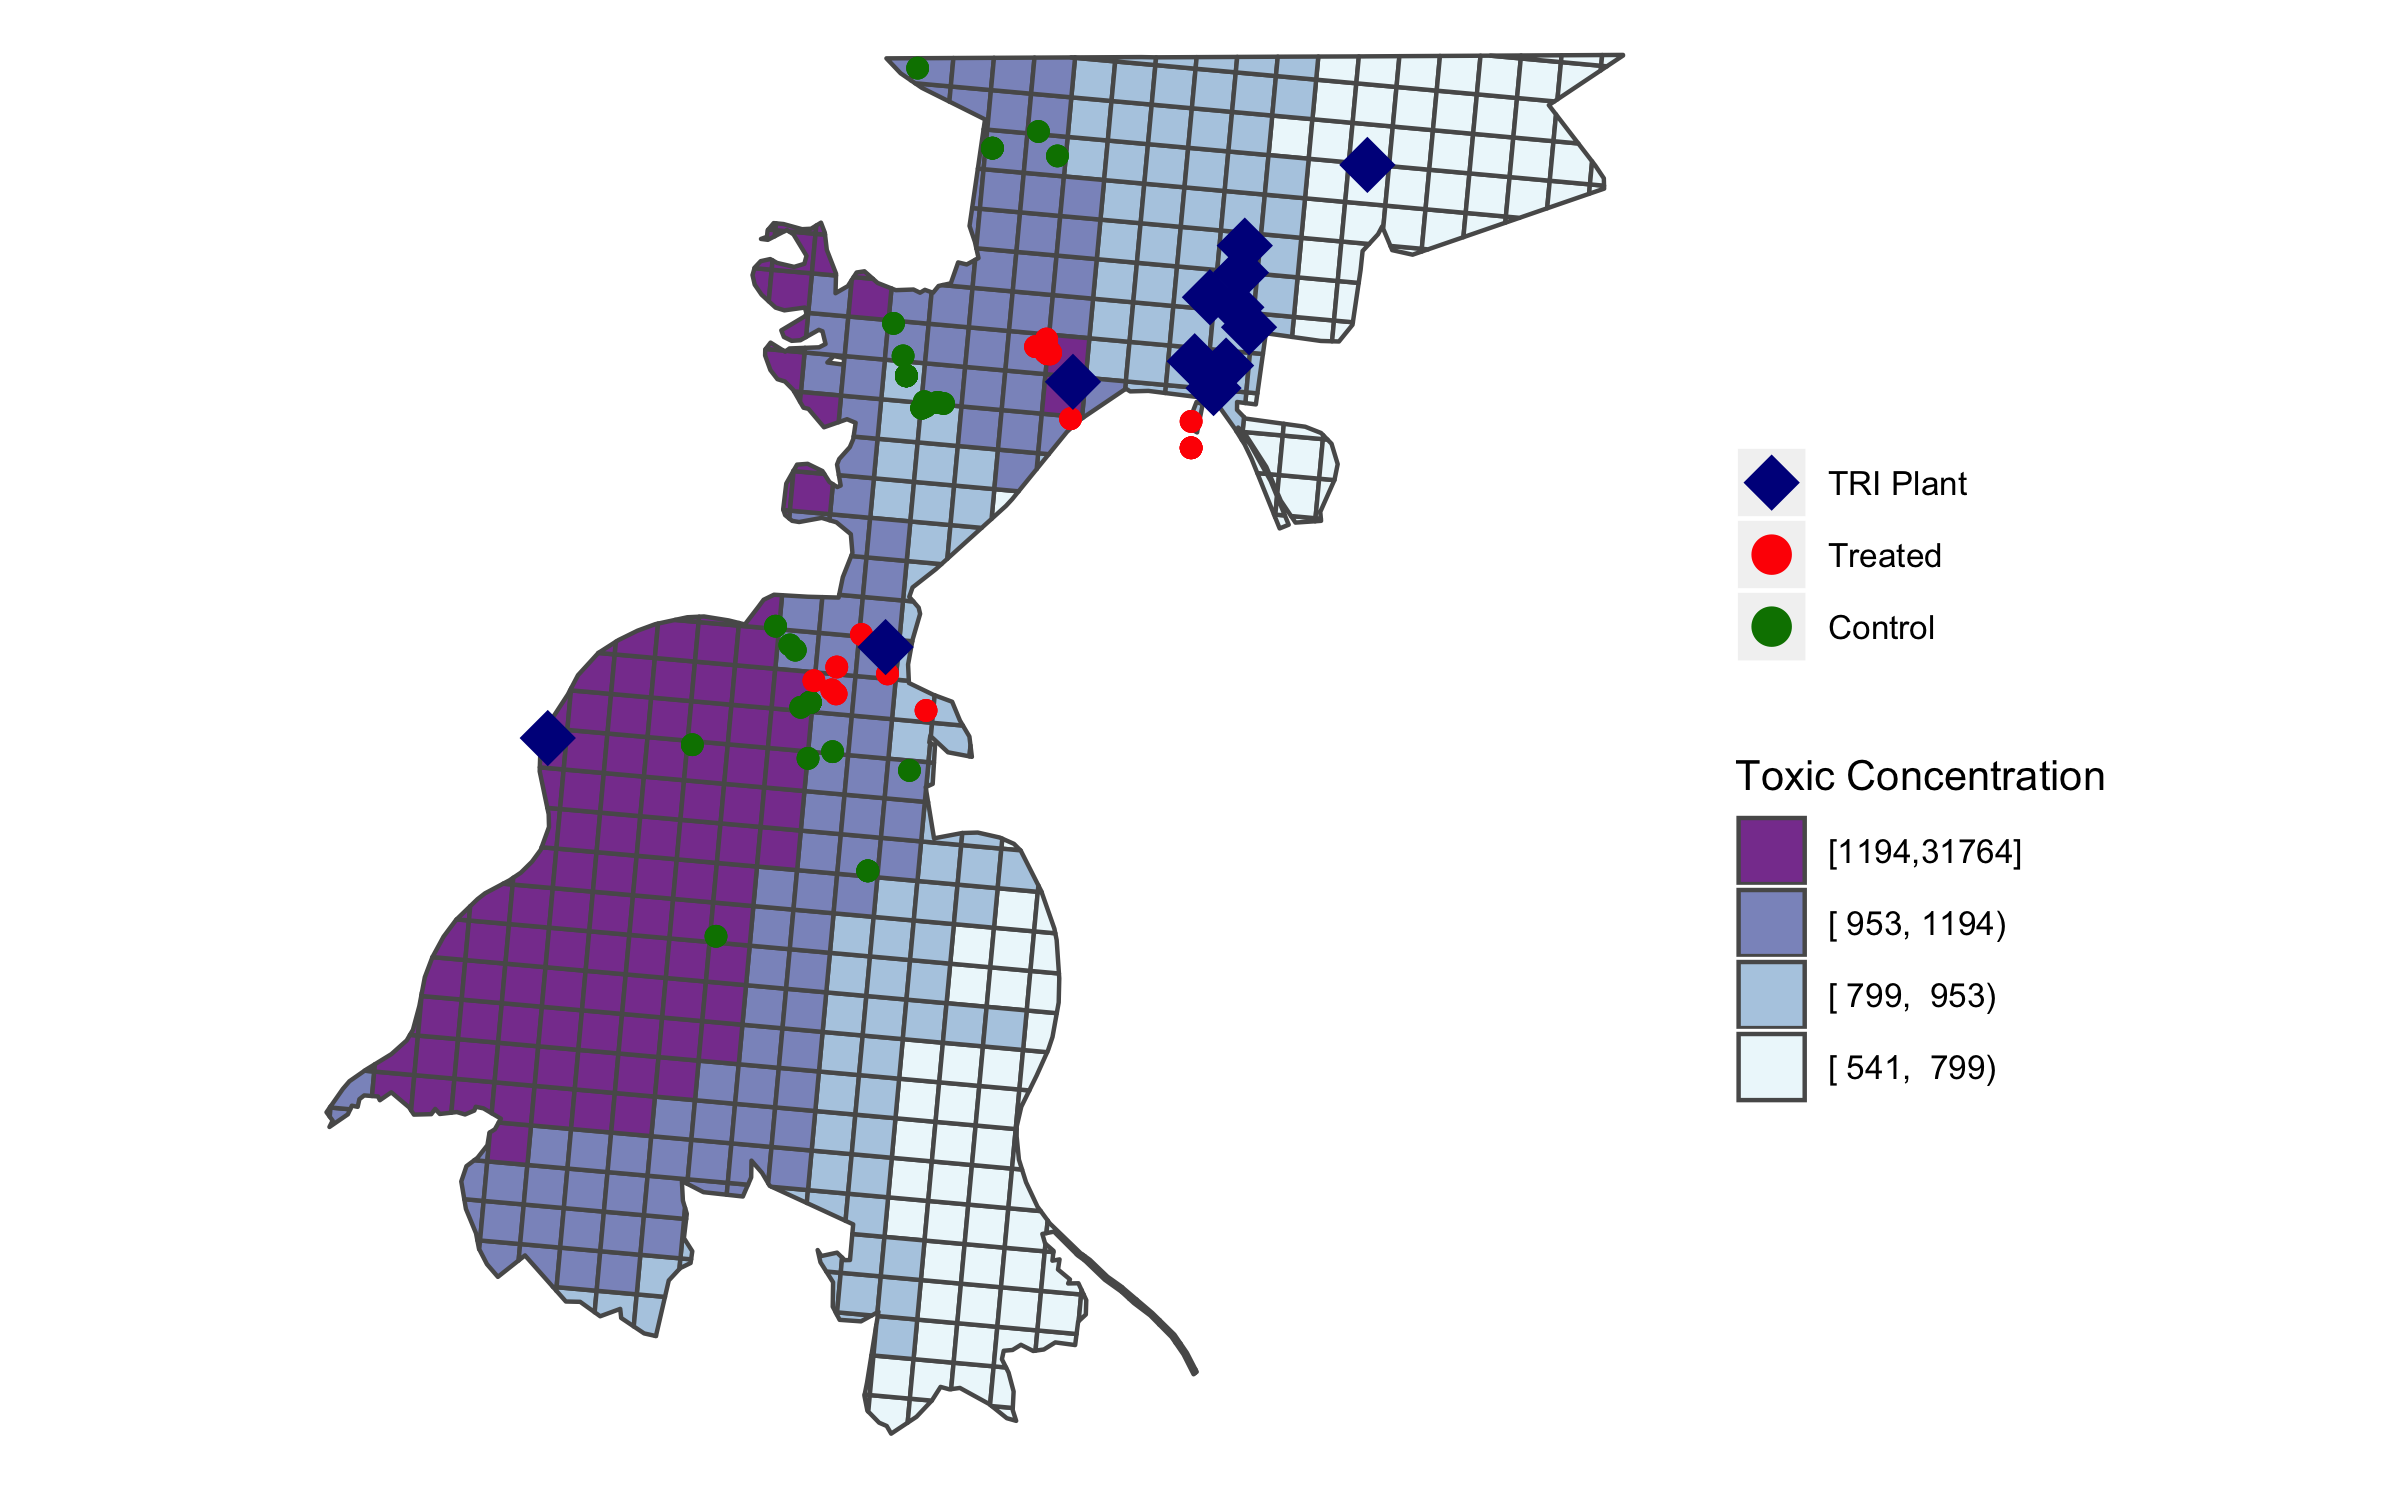
\includegraphics[scale=0.08]{figures/ZIP_B.png}

\end{subfigure}
  \\
  \tiny Christensen,Sarmiento-Barbieri,  \& Timmins (2020)
\end{figure}


\end{frame}
%----------------------------------------------------------------------%
\begin{frame}[fragile]
\frametitle{Types of Spatial Data: Rasters}


\begin{figure}[H] \centering
  \centering
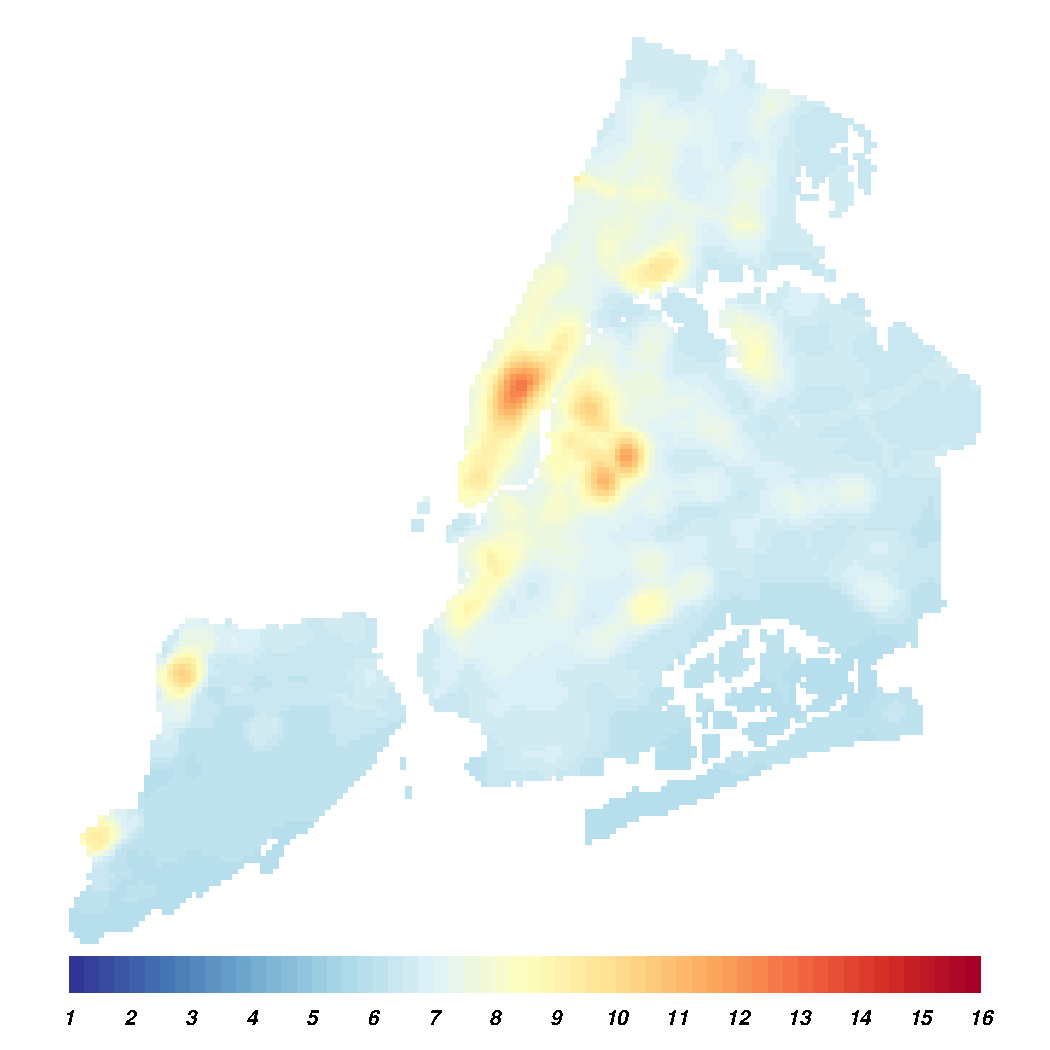
\includegraphics[scale=0.40]{figures/NewYork.pdf}
  \\
  \tiny Source:\url{https://data.cityofnewyork.us/Environment/NYCCAS-Air-Pollution-Rasters/q68s-8qxv}
\end{figure}



\end{frame}


%----------------------------------------------------------------------%
\subsection{Projections}
%----------------------------------------------------------------------%
\begin{frame}[fragile]
\frametitle{The earth ain't flat}
\begin{itemize}
	\footnotesize
	\item The world is an irregularly shaped ellipsoid, but plotting devices are flat
	\medskip
	\item But if you want to show it on a flat map you need a map projection
	\medskip
	\item This  will determine how to transform and distort latitudes and longitudes to preserve some of the map properties: area, shape, distance, direction, or bearing
\end{itemize}

\begin{figure}[H] \centering
            \captionsetup{justification=centering}
				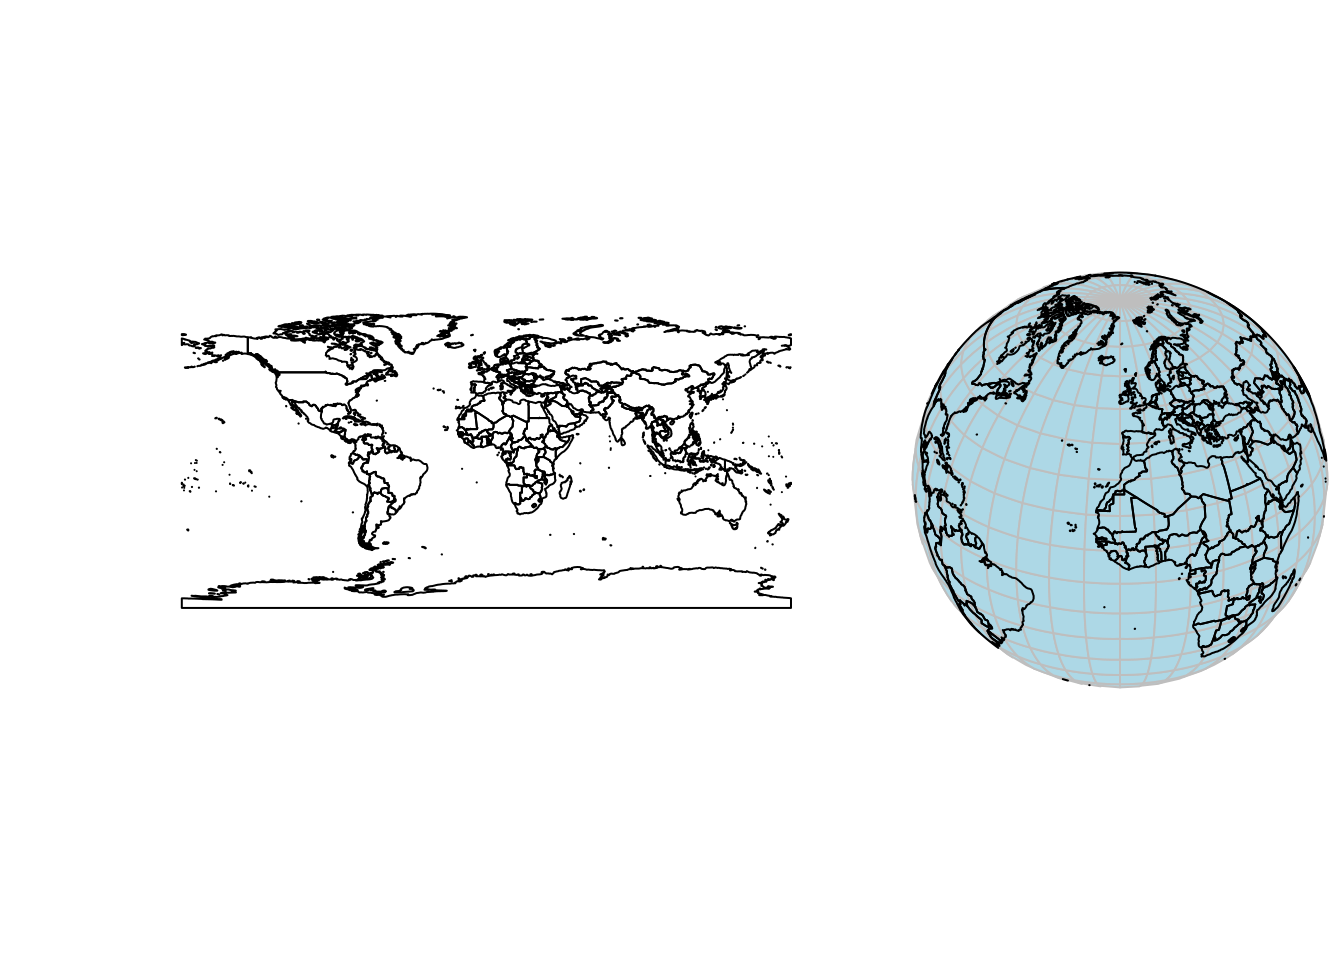
\includegraphics[scale=0.6]{figures/world-1.png}
 \end{figure}

\end{frame}
%----------------------------------------------------------------------%
\begin{frame}[fragile]
\frametitle{The earth ain't flat}
\begin{itemize}
	\footnotesize
	\item For example, sailors use Mercator projection where meridians and parallels cross each other always at the same 90 degrees angle.
	\medskip
	\item It allows to easy locate yourself on the line showing direction in which you sail
	\medskip
	\item But the projection do not preserve  distances
\end{itemize}
 

\begin{figure}[H] \centering
            \captionsetup{justification=centering}
				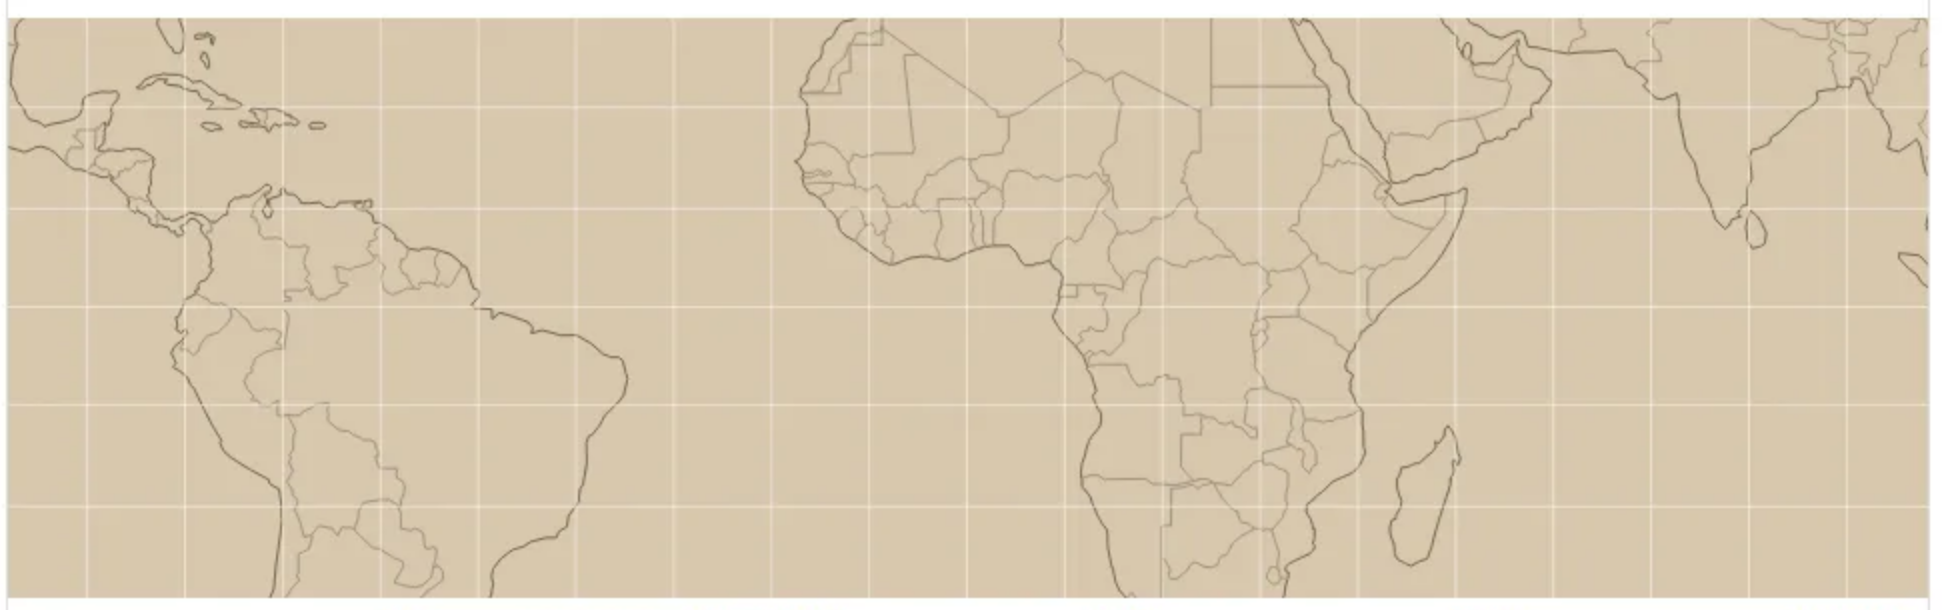
\includegraphics[scale=0.3]{figures/Mercator}
				\\
				\tiny
				Source: \url{https://www.geoawesomeness.com/all-map-projections-in-compared-and-visualized/}
 \end{figure}


\end{frame}

%----------------------------------------------------------------------%
\begin{frame}[fragile]
\frametitle{Which projection should I choose?}

\begin{itemize}
\small
\item “There exist no all-purpose projections, all involve distortion when far from the center of the specified frame” (Bivand, Pebesma, and Gómez-Rubio 2013)
\medskip
   \item  Geographic coordinate systems: coordinate systems that span the entire globe (e.g. latitude / longitude).
   \begin{itemize}
   	\footnotesize
    \item For geographic CRSs, the answer is often WGS84
    \item WGS84 is the most common CRS in the world,  EPSG code: 4326. 
   \end{itemize}
   \medskip
   \item  Projected coordinate systems: coordinate systems that are localized to minimize visual distortion in a particular region (e.g. Robinson, UTM, State Plane)
\begin{itemize}
	\footnotesize
    \item In some cases, it is not something that we are free to decide: “often the choice of projection is made by a public mapping agency” (Bivand, Pebesma, and Gómez-Rubio 2013).
    \item  This means that when working with local data sources, it is likely preferable to work with the CRS in which the data was provided.
    \item For Bogotá the IGAC promotes the adoption of MAGNA-SIRGAS. EPSG code: 4626
    \end{itemize}




\end{itemize}
\end{frame}
%----------------------------------------------------------------------%
\section{Spatial Econometrics}
\subsection{Motivation}
%----------------------------------------------------------------------%
\begin{frame}[fragile]
\frametitle{Spatial Econometrics: Motivation}


\begin{minipage}[t]{0.52\linewidth}

\begin{align}
        y = X\beta + u \nonumber
    \end{align}
\begin{itemize}
    
  
  \small
  \item Independence assumption between observation is no longer valid
  \medskip
  \item Attributes of observation $i$  may influence the attributes of observation $j$.
  \medskip
  \item We will consider various alternatives to model spatial dependence
  
  
\end{itemize}

    \end{minipage}
    \hfill
    \begin{minipage}[t]{0.43\linewidth}%
       \medskip
        \begin{figure}[H] \centering
            \captionsetup{justification=centering}
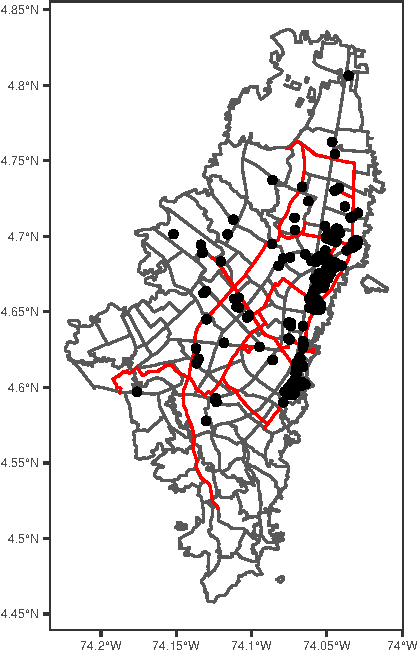
\includegraphics[scale=0.6]{figures/restaurants_bogota.pdf}

 \end{figure}
    \end{minipage}

\end{frame}


%----------------------------------------------------------------------%
\begin{frame}[fragile]
\frametitle{Spatial Econometrics: Motivation}


    \begin{minipage}[t]{0.52\linewidth}

\begin{align}
        y = X\beta + u \nonumber
    \end{align}

\begin{itemize}
    
  \small
  \item Independence assumption between observation is no longer valid
  
  \item Attributes of observation $i$  may influence the attributes of observation $j$.
  
  \item Positive Spatial correlation arises when units that are {\it close} to one another are more similar than units that are far apart
  
  \item Similarly spatial heterogeneity arises when some areas present more variability than others
\end{itemize}

    \end{minipage}
    \hfill
    \begin{minipage}[t]{0.43\linewidth}%
       \medskip
        \begin{figure}[H] 
          \begin{subfigure}{0.45\linewidth}
          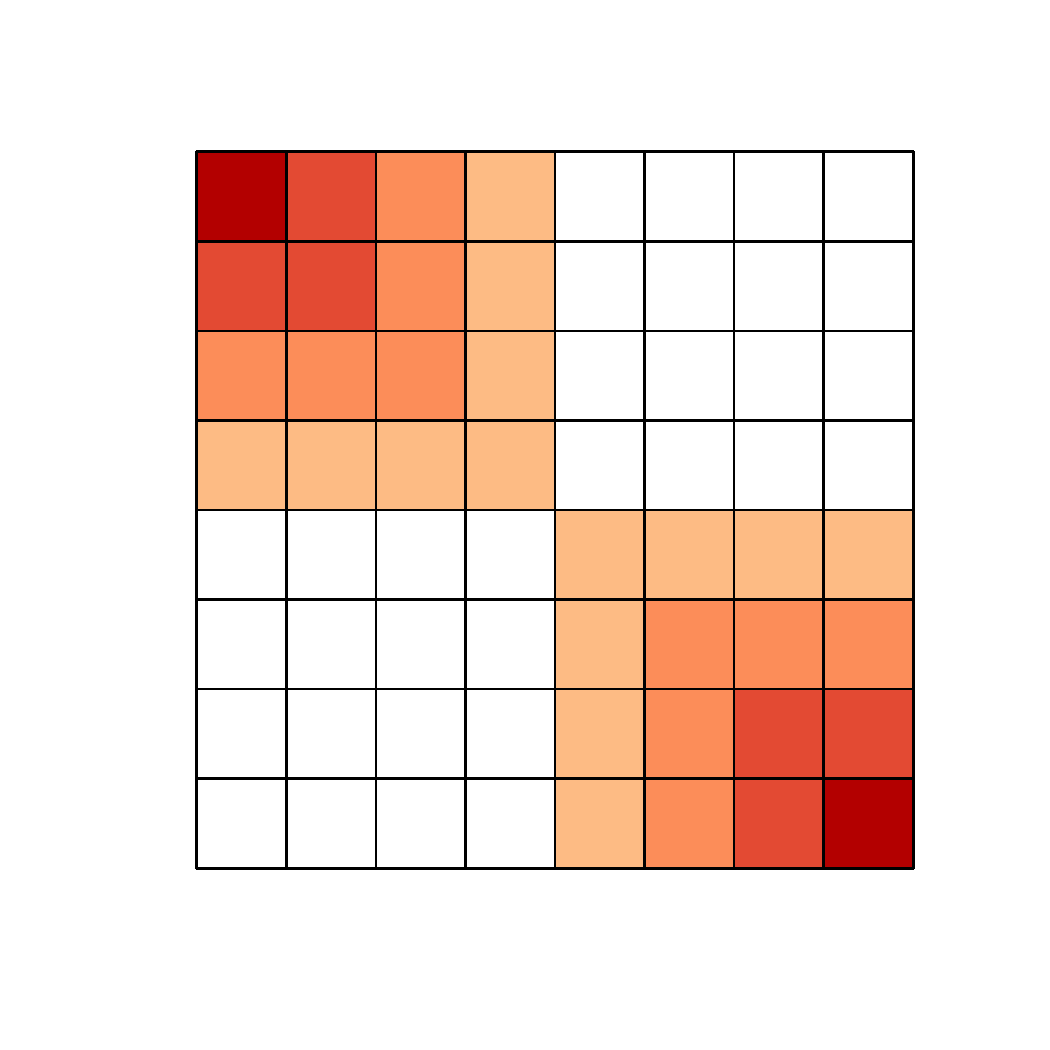
\includegraphics[scale=.21]{figures/spatial_correlation.pdf}
          \end{subfigure} \\
          
          \begin{subfigure}{0.45\linewidth}
          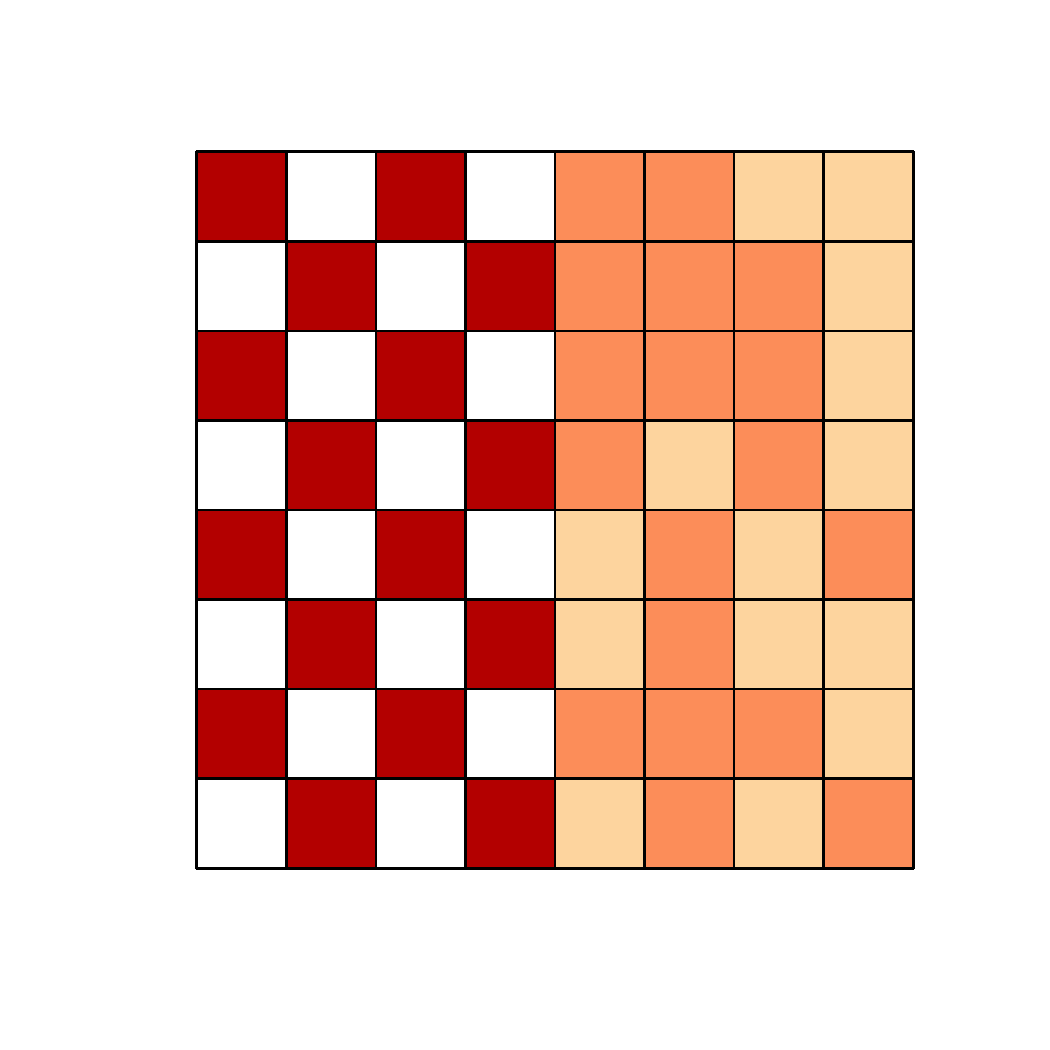
\includegraphics[scale=.21]{figures/spatial_heterogeneity.pdf}
          \end{subfigure}

  \end{figure}
    \end{minipage}

\end{frame}
%----------------------------------------------------------------------%
\subsection{Closeness }
%----------------------------------------------------------------------%
\begin{frame}[fragile]
\frametitle{Spatial Econometrics: Closeness}

 {\it “Everything is related to everything else, but close things are more related than things that are far apart”} (Tobler, 1979).

\bigskip

\begin{itemize}
  \item One of the major differences between standard econometrics and standard spatial econometrics lies, in the fact that, in order to treat spatial data, we need to use two different sets of information
  \medskip
  \begin{enumerate}
  \item Observed values of the economic variables
  \medskip
  \item Particular location where those variables are observed and to the various links of proximity between all spatial observations
  \end{enumerate}
\end{itemize}

\end{frame}
%----------------------------------------------------------------------%
\begin{frame}[fragile]
\frametitle{Spatial Econometrics: Closeness}

\bigskip

\begin{minipage}[t]{0.45\linewidth}
Rook criterion: two units are close to one another if they share a side
  \begin{figure}[H] \centering
    \captionsetup{justification=centering}
    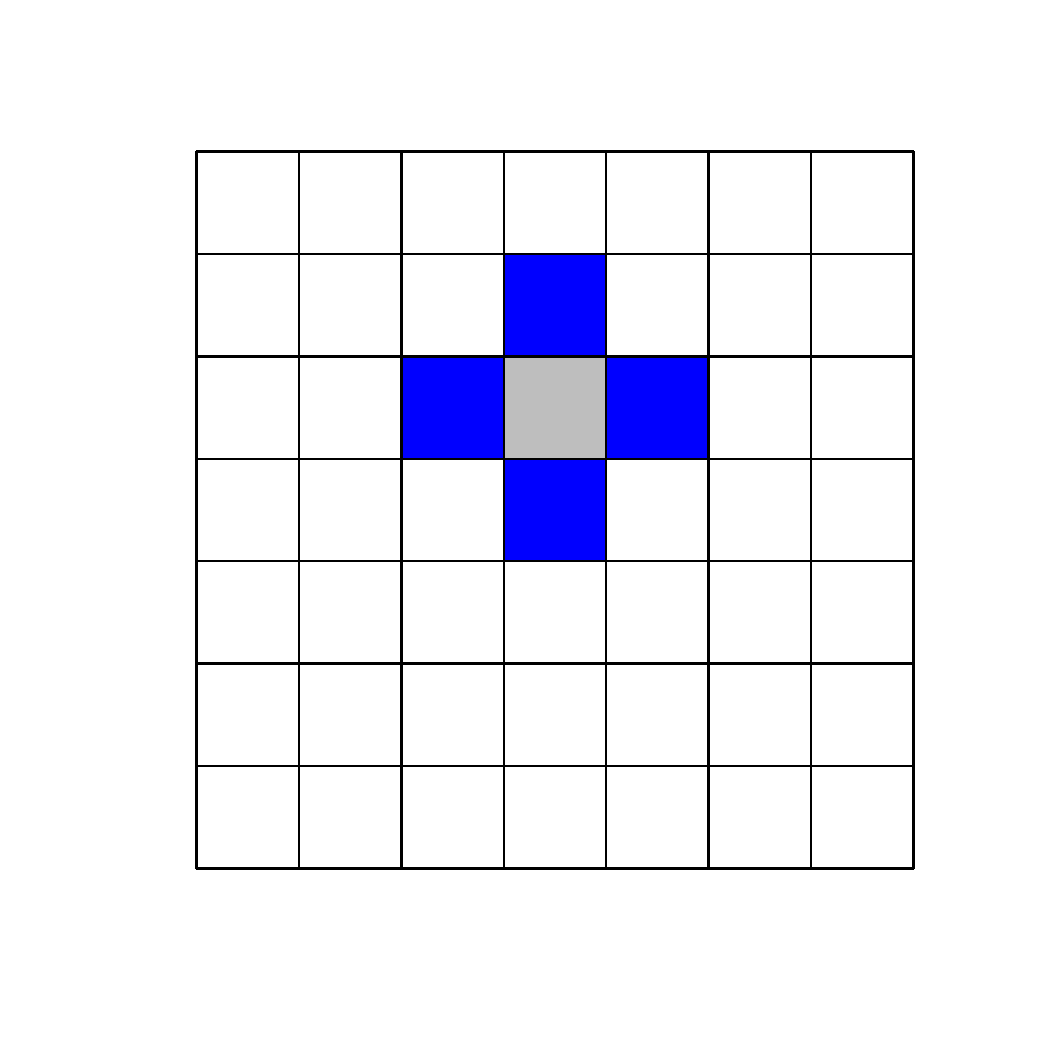
\includegraphics[scale=0.3]{figures/rook.pdf}
   \end{figure}
  
    \end{minipage}
    \hfill
\begin{minipage}[t]{0.45\linewidth}%
Queen criterion: two units are close if they share a side or an edge.
  \begin{figure}[H] \centering
    \captionsetup{justification=centering}
    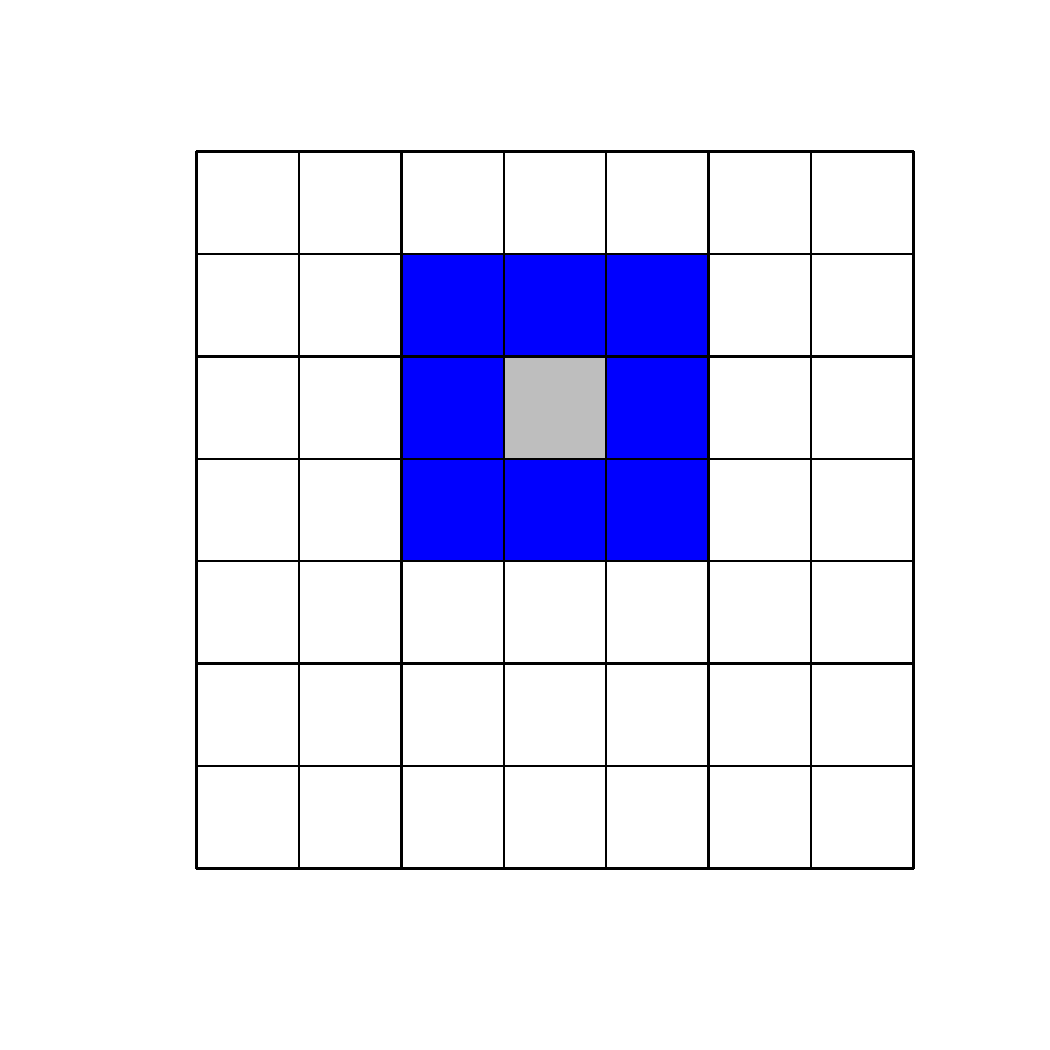
\includegraphics[scale=0.3]{figures/queen.pdf}
   \end{figure}
\end{minipage}


\end{frame}

%----------------------------------------------------------------------%
\subsection{Weights Matrix}
%----------------------------------------------------------------------%
\begin{frame}[fragile]
\frametitle{Spatial Econometrics: Weights Matrix}

\begin{itemize}
  \item At the heart of traditional spatial econometrics is the definition of the {\it weights matrix}:
\end{itemize}


\begin{align}
W=\left(\begin{array}{cccc}
w_{11} & \dots & \dots & w_{n1}\\
\vdots & w_{ij} &  & \vdots\\
\vdots &  & \ddots & \vdots\\
w_{n_{1}} & \dots & \dots & w_{nn}
\end{array}\right)_{n\times n}
\end{align}

with generic element:

\begin{equation}
w_{ij}=\begin{cases}
1 & if\,j\in N\left(i\right)\\
0 & o.w
\end{cases}
\end{equation}

$N(i)$ being the set of neighbors of location $j$. By convention, the diagonal elements are set to zero, i.e. $w_{ii}=0$. 

\end{frame}
%----------------------------------------------------------------------%
\begin{frame}[fragile]
\frametitle{Spatial Econometrics: Weights Matrix}



\begin{itemize}
\item The specification of  the neighboring set ($N(i)$) is quite arbitrary and there's a wide range of suggestions in the literature. 
\bigskip
  \begin{itemize}
    \item Rook criterion
    \medskip
    \item Queen criterion
    \medskip
    \item Two observations are neighbors if they are within a certain distance, i.e., $j\in N(i)$ if $d_{ij} < d_{max}$ where $d$ is the distance between location $i$ and $j$. 
    \medskip
    \item Closest neighbor, ties can be solved randomly
    \medskip
    \item More general matrices can also be specified by considering entries of $w_{ij}$ as functions of geographical, economic or social distances between areas rather than simply characterized by dichotomous entries 
  \end{itemize}
\end{itemize}


\end{frame}

%----------------------------------------------------------------------%
\begin{frame}[fragile]
\frametitle{Some Examples of Weights Matrices}


\begin{minipage}[t]{0.53\linewidth}
  \begin{figure}[H] \centering
    \captionsetup{justification=centering}
    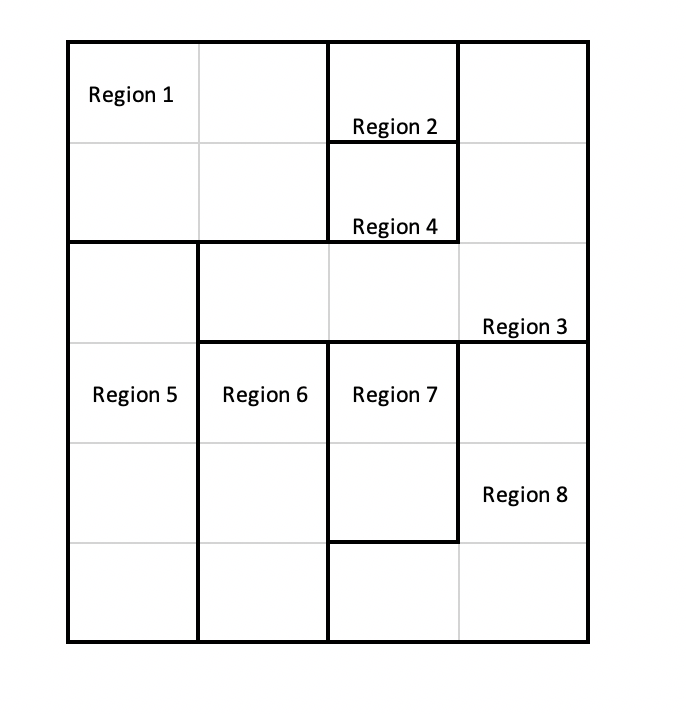
\includegraphics[scale=0.6]{figures/regions_example}
   \end{figure}
  
    \end{minipage}
    \hfill
\begin{minipage}[t]{0.43\linewidth}%
\scriptsize
Adjacency Criterion
\begin{align}
W=\left(\begin{array}{cccccccc}
0 & 1 & 1 & 1 & 1 & 0 & 0 & 0\\
1 & 0 & 1 & 1 & 0 & 0 & 0 & 0\\
1 & 1 & 0 & 1 & 1 & 1 & 1 & 1\\
1 & 1 & 1 & 0 & 0 & 0 & 0 & 0\\
1 & 0 & 1 & 0 & 0 & 1 & 0 & 0\\
0 & 0 & 1 & 0 & 1 & 0 & 1 & 1\\
0 & 0 & 1 & 0 & 0 & 1 & 0 & 1\\
0 & 0 & 1 & 0 & 0 & 1 & 1 & 0
\end{array}\right)_{8\times8} \nonumber
\end{align}
\end{minipage}

\end{frame}
%----------------------------------------------------------------------%
\begin{frame}[fragile]
\frametitle{Some Examples of Weights Matrices}


\begin{minipage}[t]{0.53\linewidth}
  \begin{figure}[H] \centering
    \captionsetup{justification=centering}
    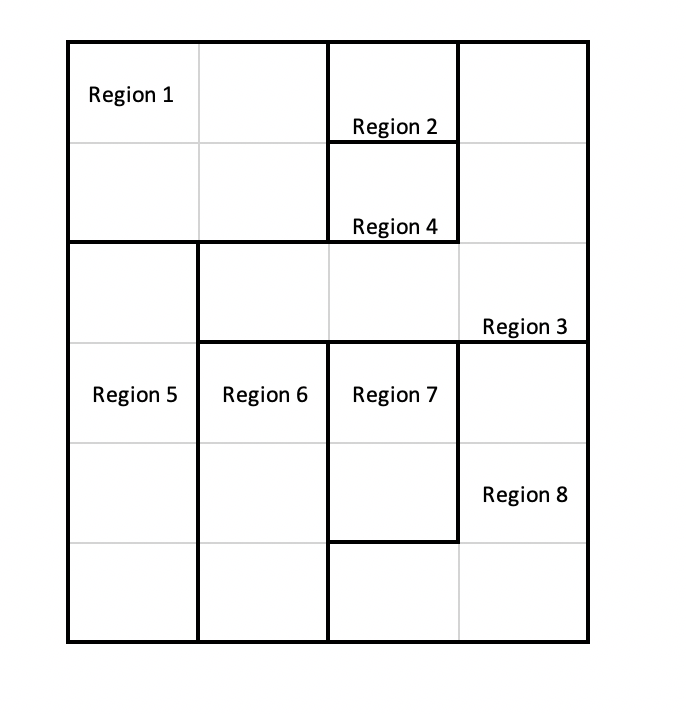
\includegraphics[scale=0.6]{figures/regions_example}
   \end{figure}
  
    \end{minipage}
    \hfill
\begin{minipage}[t]{0.43\linewidth}%
\scriptsize
Nearest Neighbor
\begin{align}
W=\left(\begin{array}{cccccccc}
0 & 1 & 0 & 0 & 0 & 0 & 0 & 0\\
0 & 0 & 0 & 1 & 0 & 0 & 0 & 0\\
0 & 0 & 0 & 1 & 0 & 0 & 0 & 0\\
0 & 1 & 0 & 0 & 0 & 0 & 0 & 0\\
0 & 0 & 0 & 0 & 0 & 1 & 0 & 0\\
0 & 0 & 0 & 0 & 0 & 0 & 1 & 0\\
0 & 0 & 0 & 0 & 0 & 1 & 0 & 0\\
0 & 0 & 0 & 0 & 0 & 0 & 1 & 0
\end{array}\right)_{8\times8} \nonumber
\end{align}
\end{minipage}


\end{frame}
%----------------------------------------------------------------------%
\begin{frame}[fragile]
\frametitle{Some Examples of Weights Matrices}


\begin{minipage}[t]{0.53\linewidth}
  \begin{figure}[H] \centering
    \captionsetup{justification=centering}
    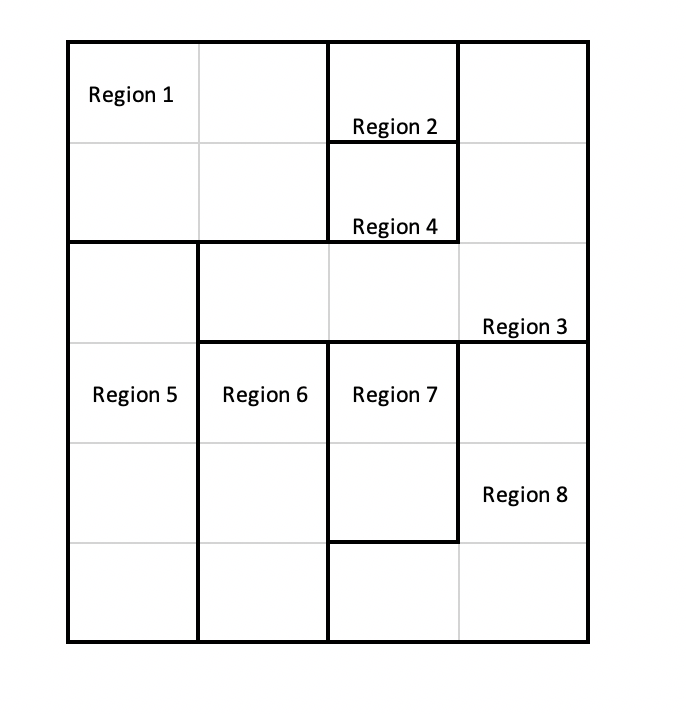
\includegraphics[scale=0.6]{figures/regions_example}
   \end{figure}
  
    \end{minipage}
    \hfill
\begin{minipage}[t]{0.43\linewidth}%
\scriptsize
Distance $<2$
\begin{align}
W=\left(\begin{array}{cccccccc}
0 & 1 & 0 & 1 & 0 & 0 & 0 & 0\\
1 & 0 & 1 & 1 & 0 & 0 & 0 & 0\\
0 & 1 & 0 & 1 & 0 & 0 & 0 & 0\\
1 & 1 & 1 & 0 & 0 & 0 & 0 & 0\\
0 & 0 & 0 & 0 & 0 & 1 & 1 & 0\\
0 & 0 & 0 & 0 & 1 & 0 & 1 & 0\\
0 & 0 & 0 & 0 & 1 & 1 & 0 & 0\\
0 & 0 & 0 & 0 & 0 & 0 & 1 & 0
\end{array}\right)_{8\times8} \nonumber
\end{align}
\end{minipage}

\end{frame}

%----------------------------------------------------------------------%
\begin{frame}[fragile]
\frametitle{Some Examples of Weights Matrices}


  \begin{figure}[H] \centering
    \captionsetup{justification=centering}
    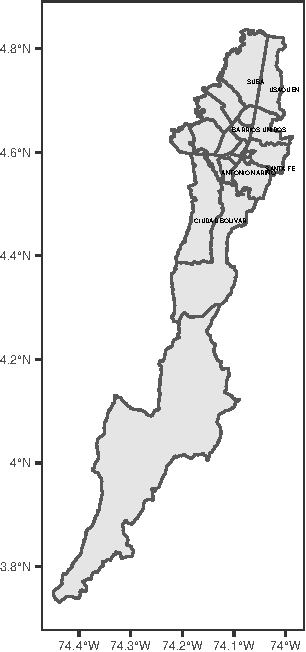
\includegraphics[scale=0.6]{figures/localities.pdf}
   \end{figure}

\end{frame}

%----------------------------------------------------------------------%
\begin{frame}[fragile]
\frametitle{Some Examples of Weights Matrices}

  \begin{figure}[H] \centering
    \captionsetup{justification=centering}
    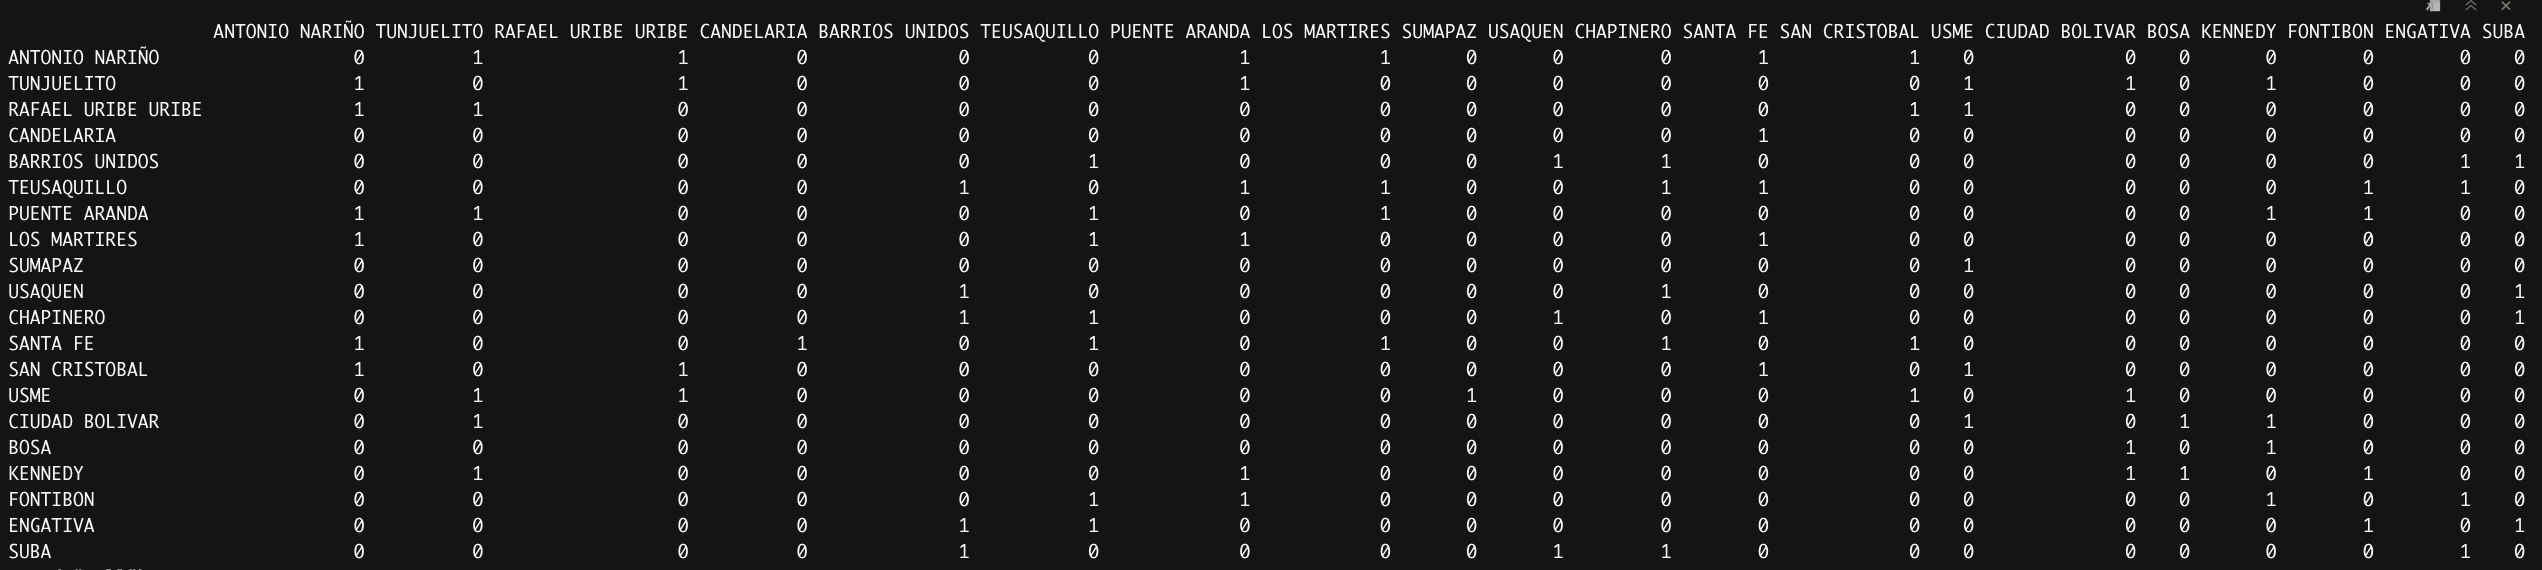
\includegraphics[scale=0.35]{figures/matrix_loc}
   \end{figure}

\end{frame}


%----------------------------------------------------------------------%
\begin{frame}[fragile]
\frametitle{Some Examples of Weights Matrices}
Quite often the $W$ matrices are standardized to sum to one in each row

\begin{align}
w^*_{ij}=\frac{w_{ij}}{\sum_{j=1}^n w_{ij}}
\end{align}

This can be quite useful since $L(y) =W^{*} y$ in which each single element is equal to

\begin{align}
L(y_i) &= \sum_{j=1}^n w^*_{ij}y_j \\ \nonumber
&= \sum_{j=1}^n \frac{w_{ij}y_j}{\sum_{j=1}^n w_{ij}}  \\
&= \frac{\sum_{j\in N(i)}y_j}{\# N(i)}
\end{align}
\end{frame}
%----------------------------------------------------------------------%
\begin{frame}[fragile]
\frametitle{Some Examples of Weights Matrices}

  \begin{figure}[H] \centering
    \captionsetup{justification=centering}
    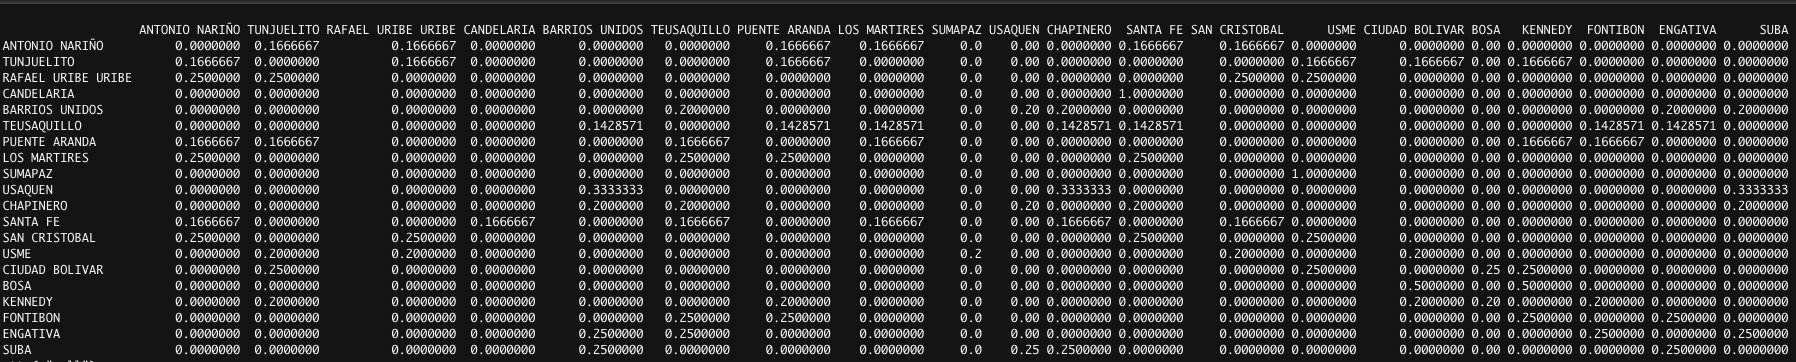
\includegraphics[scale=0.45]{figures/matrix_loc_row_stand}
   \end{figure}

\end{frame}

%----------------------------------------------------------------------%
\begin{frame}[fragile]
\frametitle{Some Examples of Weights Matrices}


  \begin{figure}[H] \centering
    \captionsetup{justification=centering}
    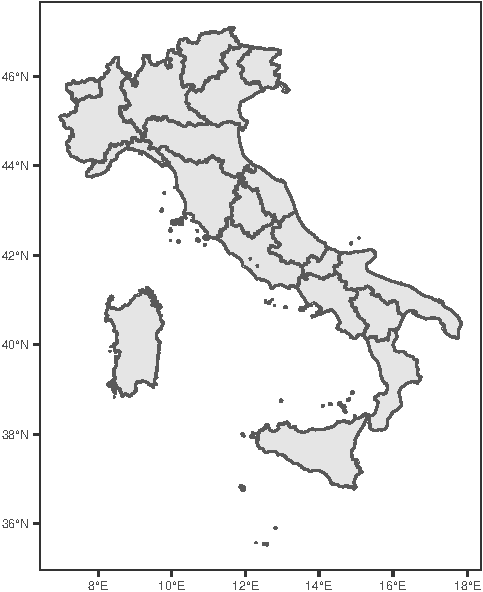
\includegraphics[scale=0.6]{figures/italia.pdf}
   \end{figure}

\end{frame}

%----------------------------------------------------------------------%
\begin{frame}[fragile]
\frametitle{Some Examples of Weights Matrices}


  \begin{figure}[H] \centering
    \captionsetup{justification=centering}
    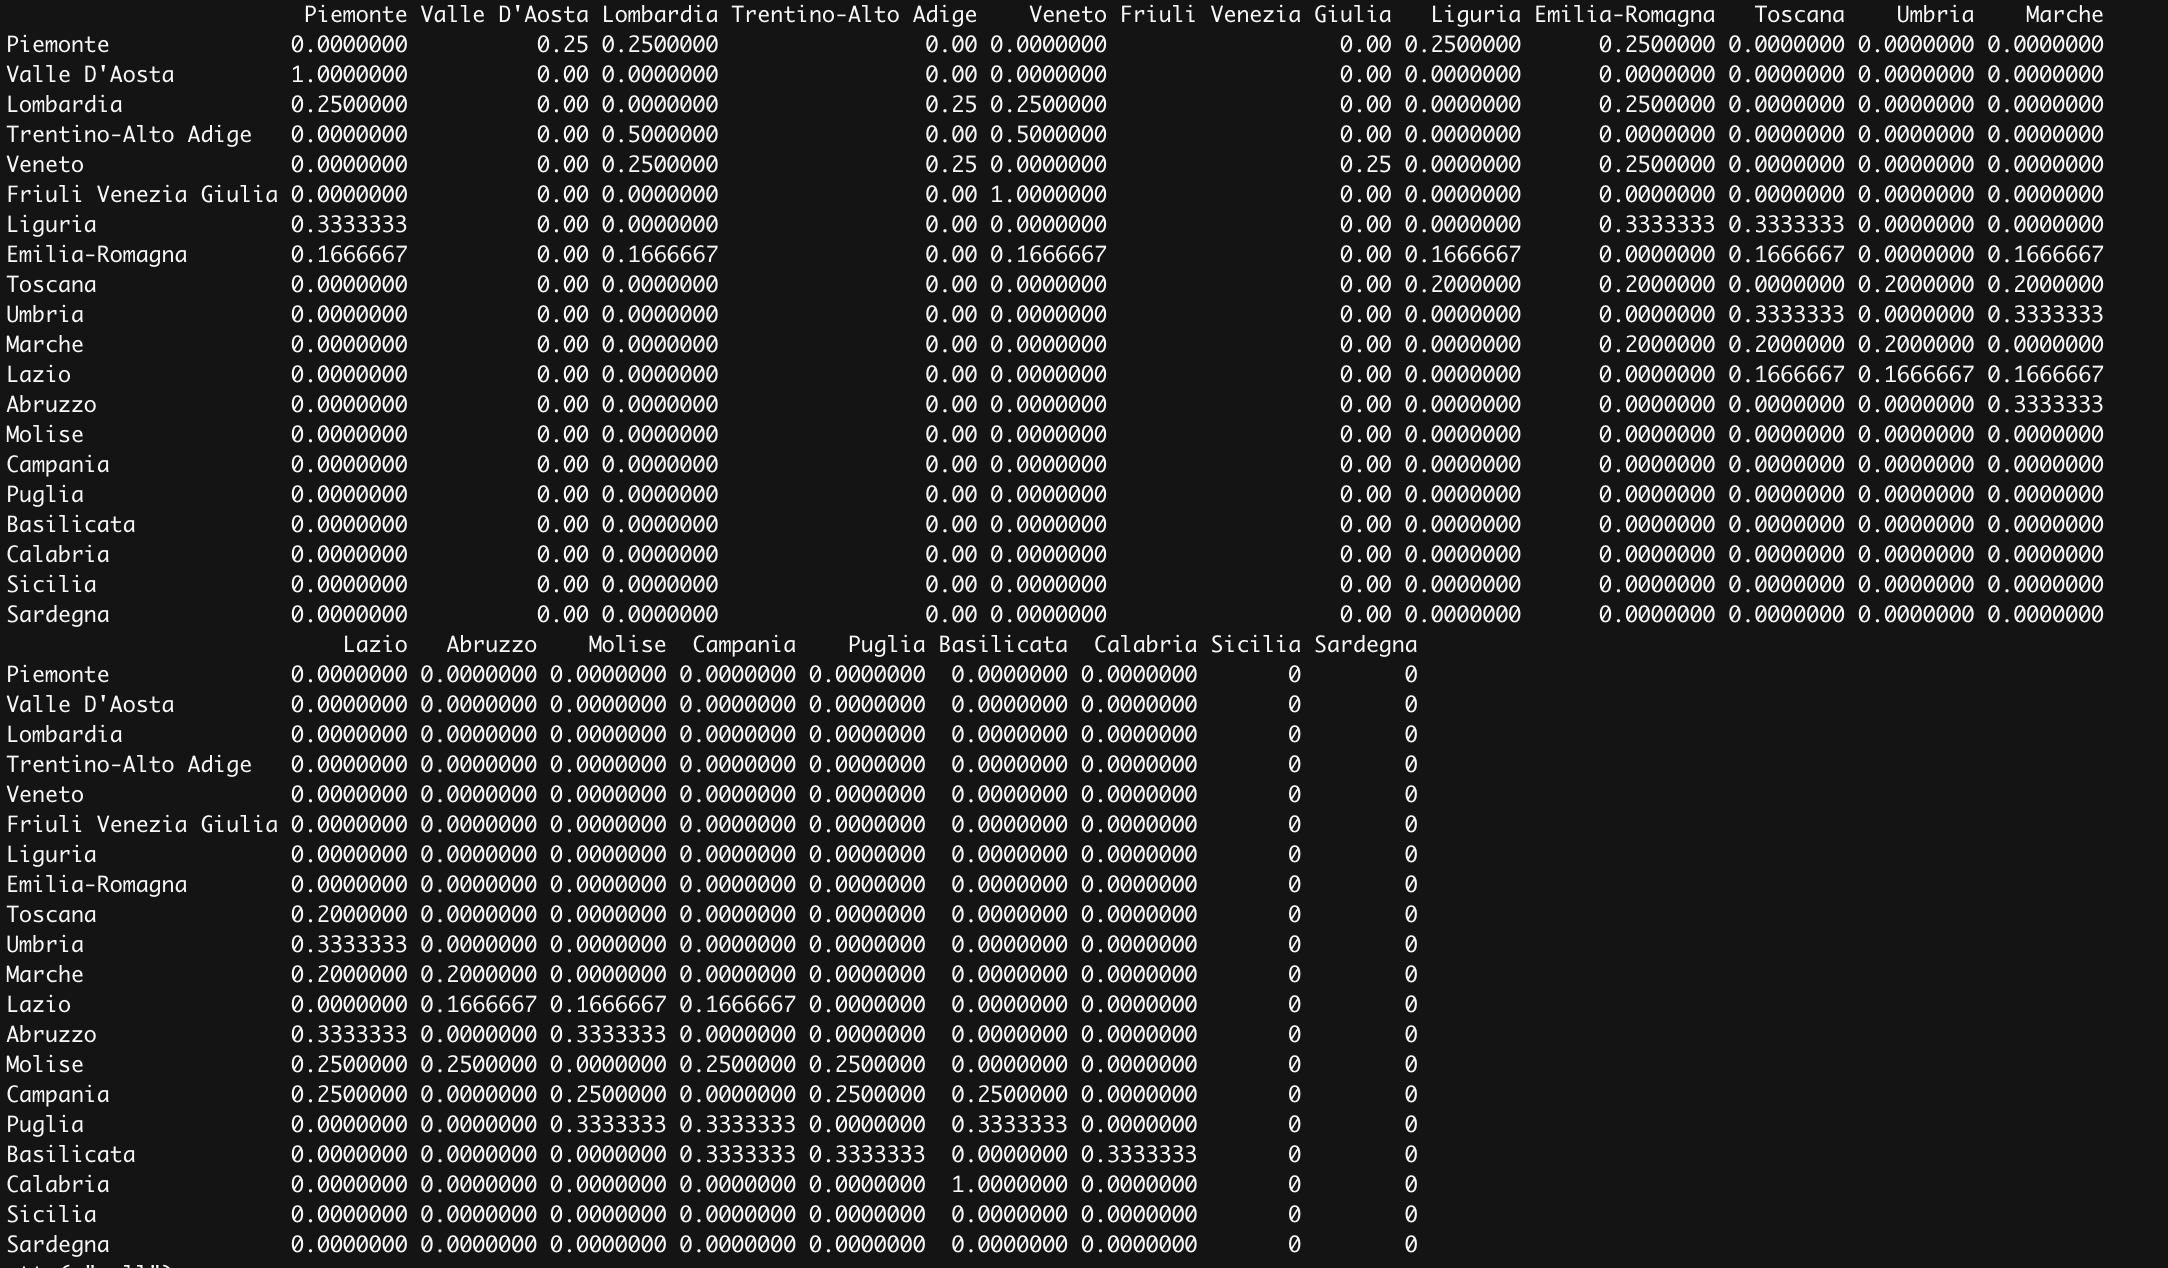
\includegraphics[scale=0.3]{figures/mat_italia}
   \end{figure}


\end{frame}
%----------------------------------------------------------------------%
\subsection{Spatial Regresion in R}
%----------------------------------------------------------------------%
\begin{frame}[fragile]
\frametitle{Spatial Regressions }
\framesubtitle{Spatial Autoregressive (SAR) Models}

\begin{itemize}
\item Spatial lag dependence in a regression setting can be modeled similar to
an autoregressive process in time series. Formally,
\end{itemize}


\[ y= \rho Wy+ X \beta + \epsilon \]

\begin{itemize}
  \footnotesize
\item \(Wy\) induces a nonzero correlation with the error term, similar to the presence of an endogenous variable (OVB).

\item  Unlike to time series, \(Wy_i\) is always correlated with \(\epsilon_i\) 

\item OLS estimates in the non spatial model will be biased and inconsistent. (Anselin and Bera, 1998)

\item The estimation of the SAR model can be approached in two ways.
\begin{enumerate}
  \tiny
  \item Assume normality of the error term and use maximum likelihood.
  \item Use 2SLS
\end{enumerate}
\item In \texttt{R}  the function \texttt{lagsarlm} uses MLE
\end{itemize}


\end{frame}


%----------------------------------------------------------------------%
\begin{frame}[fragile]
\frametitle{Spatial Regresion in R}

\footnotesize
\begin{itemize}
    \item Example crime, foreclosures, and unemployment
    \item Load Packages
\end{itemize}
\begin{tiny}
\begin{Shaded}
\begin{Highlighting}[]
\FunctionTok{require}\NormalTok{(}\StringTok{"spdep"}\NormalTok{)}
\FunctionTok{require}\NormalTok{(}\StringTok{"spatialreg"}\NormalTok{)}
\FunctionTok{require}\NormalTok{(}\StringTok{"stargazer"}\NormalTok{)}
\end{Highlighting}
\end{Shaded}
\end{tiny}

\begin{itemize}
    \item OLS
\end{itemize}

\begin{Shaded}
\begin{tiny}
\begin{Highlighting}[]
\NormalTok{ols}\OtherTok{\textless{}{-}}\FunctionTok{lm}\NormalTok{(violent}\SpecialCharTok{\textasciitilde{}}\NormalTok{est\_fcs\_rt}\SpecialCharTok{+}\NormalTok{bls\_unemp, }\AttributeTok{data=}\NormalTok{chi.poly)}
\end{Highlighting}
\end{tiny}
\end{Shaded}



\begin{itemize}
    \item SAR model
\end{itemize}

\begin{Shaded}
\begin{tiny}
\begin{Highlighting}[]
\NormalTok{list.queen}\OtherTok{\textless{}{-}}\FunctionTok{poly2nb}\NormalTok{(chi.poly, }\AttributeTok{queen=}\ConstantTok{TRUE}\NormalTok{)}
\NormalTok{W}\OtherTok{\textless{}{-}}\FunctionTok{nb2listw}\NormalTok{(list.queen, }\AttributeTok{style=}\StringTok{"W"}\NormalTok{, }\AttributeTok{zero.policy=}\ConstantTok{TRUE}\NormalTok{)}
\NormalTok{W}
\NormalTok{sar.chi}\OtherTok{\textless{}{-}}\FunctionTok{lagsarlm}\NormalTok{(violent}\SpecialCharTok{\textasciitilde{}}\NormalTok{est\_fcs\_rt}\SpecialCharTok{+}\NormalTok{bls\_unemp, }\AttributeTok{data=}\NormalTok{chi.poly, W)}
\end{Highlighting}
\end{tiny}
\end{Shaded}

\end{frame}


%----------------------------------------------------------------------%
\begin{frame}[fragile]
\frametitle{Spatial Regresion in R}
\begin{tiny}
\begin{Shaded}
\begin{Highlighting}[]
\FunctionTok{stargazer}\NormalTok{(ols,sar.chi, }\AttributeTok{header=}\ConstantTok{FALSE}\NormalTok{, }\AttributeTok{type=}\StringTok{"latex"}\NormalTok{)}
\end{Highlighting}
\end{Shaded}
\end{tiny}

\begin{table}[H] \centering 
  \small
\begin{tabular}{@{\extracolsep{5pt}}lcc} 
\\[-1.8ex]\hline 
\hline \\[-1.8ex] 
 & \multicolumn{2}{c}{\textit{Dependent variable:}} \\ 
\cline{2-3} 
\\[-1.8ex] & \multicolumn{2}{c}{Violent Crime} \\ 
\\[-1.8ex] & \textit{OLS} & \textit{SAR} \\ 
\\[-1.8ex] & (1) & (2)\\ 
\hline \\[-1.8ex] 
 Foreclosures & 28.298$^{***}$ & 15.682$^{***}$ \\ 
  & (1.435) & (1.560) \\ 
 Unemployment & $-$0.308 & 8.895$^{*}$ \\ 
  & (5.770) & (5.245) \\ 
 Constant & $-$18.627 & $-$93.789$^{**}$ \\ 
  & (45.366) & (41.316) \\ 
\hline \\[-1.8ex] 
Observations & 897 & 897 \\ 
\hline 
\hline \\[-1.8ex] 
\textit{Note:}  & \multicolumn{2}{r}{$^{*}$p$<$0.1; $^{**}$p$<$0.05; $^{***}$p$<$0.01} \\ 
\end{tabular} 
\end{table}




\end{frame}
%----------------------------------------------------------------------%
\begin{frame}

\frametitle{Review \& Next Steps}
  
  \begin{itemize} 
    \item Today:
    \medskip
    \begin{itemize} 
        \item Closeness
        \medskip
        \item Weights Matrix
        \medskip
        \item Examples of Weight Matrices Weights Matrix in R
        \medskip
        \item  Spatial Regressions (SAR Models)
      \end{itemize}
    \bigskip  

  \item  Next class: More on Spatial Regressions



\end{itemize}
\end{frame}

%----------------------------------------------------------------------%
\section{Further Readings}
%----------------------------------------------------------------------%
\begin{frame}
\frametitle{Further Readings (I)}
\scriptsize
\begin{itemize}

  \item Albouy, D., Christensen, P., \& Sarmiento-Barbieri, I. (2020). Unlocking amenities: Estimating public good complementarity. Journal of Public Economics, 182, 104110. 
  \medskip
  \item Anselin, Luc, \& Anil K Bera. 1998. “Spatial Dependence in Linear Regression Models with an Introduction to Spatial Econometrics.” Statistics Textbooks and Monographs 155. MARCEL DEKKER AG: 237–90.
  \medskip
  \item Arbia, G. (2014). A primer for spatial econometrics with applications in R. Palgrave Macmillan. (Chapters 2 and 3)
  \medskip
  \item Bivand, R. S.,  \& Pebesma, E. J. (2020). Spatial Data Science \url{https://keen-swartz-3146c4.netlify.app/} (Chapter 8)
  \medskip
  \item Bivand, R. S., Gómez-Rubio, V., \& Pebesma, E. J. (2008). Applied spatial data analysis with R (Vol. 747248717, pp. 237-268). New York: Springer.
  \medskip
  \item Blumenstock, J., Cadamuro, G., \& On, R. (2015). Predicting poverty and wealth from mobile phone metadata. Science, 350(6264), 1073-1076.
  \medskip
  \item Christensen, P.,  Sarmiento-Barbieri, I., Timmins C. (2020). Housing Discrimination and the Pollution Exposure Gap in the United States. NBER WP No. 26805
  \medskip
  \item Lee, K., \& Braithwaite, J. (2020). High-Resolution Poverty Maps in Sub-Saharan Africa. arXiv preprint arXiv:2009.00544.
  \end{itemize}
\end{frame}


%----------------------------------------------------------------------%
\begin{frame}
\frametitle{Further Readings (II)}
\scriptsize
\begin{itemize}

  \item Lovelace, R., Nowosad, J., \& Muenchow, J. (2019). Geocomputation with R. CRC Press. (Chapters 2 \& 6)
  \medskip
  \item McMillen, D., Sarmiento-Barbieri, I., \& Singh, R. (2019). Do more eyes on the street reduce Crime? Evidence from Chicago's safe passage program. Journal of urban economics, 110, 1-25.
  \medskip
  \item Sarmiento-Barbieri, I. (2016). An Introduction to Spatial Econometrics in R. \url{http://www.econ.uiuc.edu/~lab/workshop/Spatial_in_R.html}
  \medskip
  \item Tobler, WR. 1979. “Cellular Geography.” In Philosophy in Geography, 379–86. Springer.
  \medskip
  \item Wasser, L. GIS With R: Projected vs Geographic Coordinate Reference Systems \url{https://www.earthdatascience.org/courses/earth-analytics/spatial-data-r/geographic-vs-projected-coordinate-reference-systems-UTM/} Last Access September 10, 2020
\end{itemize}

\end{frame}


\section{Appendix: Spatial Basics in R}
%----------------------------------------------------------------------%
\subsection{Reading and Mapping spatial data in R}
%----------------------------------------------------------------------%
\begin{frame}[fragile]
\frametitle{Reading and Mapping spatial data in R}

\begin{itemize}
 \item Spatial data comes in various formats. 
 \medskip
 \item One of the most used format are \texttt{shapefiles}
 \medskip
 \item This type of files stores non topological geometry and attribute information for the spatial features in a data set
 \medskip
\begin{itemize}

\item Main file: file.shp
\item Index file: file.shx
\item dBASE table: file.dbf
\end{itemize}
\bigskip
\item Data comes from \url{https://datosabiertos.bogota.gov.co}
\end{itemize}
\end{frame}
%----------------------------------------------------------------------%
\begin{frame}[fragile]
\frametitle{Reading shapefiles in R}

\begin{itemize}
    \item Basic Packages
    \begin{itemize}
        \item Read and handle spatial data
        \begin{scriptsize}
        \begin{Shaded}
        \begin{Highlighting}[]
\KeywordTok{require}\NormalTok{(}\StringTok{"sf"}\NormalTok{)}
        \end{Highlighting}
        \end{Shaded}
        \end{scriptsize}
        \item Plotting and data wrangling
        \begin{scriptsize}
        \begin{Shaded}
        \begin{Highlighting}[]
\KeywordTok{require}\NormalTok{(}\StringTok{"ggplot2"}\NormalTok{)}
\KeywordTok{require}\NormalTok{(}\StringTok{"dplyr"}\NormalTok{)}
        \end{Highlighting}
        \end{Shaded}
        \end{scriptsize}
    \end{itemize}   
\end{itemize}

\begin{scriptsize}
\begin{Shaded}
\begin{Highlighting}[]
\NormalTok{bars\textless{}{-}}\KeywordTok{st\_read}\NormalTok{(}\StringTok{"egba/EGBa.shp"}\NormalTok{)}
\end{Highlighting}
\end{Shaded}

\begin{verbatim}
## Reading layer `EGBa' from data source `egba/EGBa.shp' using driver 
## `ESRI Shapefile'
## Simple feature collection with 515 features and 7 fields
## geometry type:  POINT
## dimension:      XY
## bbox:           xmin: -74.17607 ymin: 4.577897 xmax: -74.02929 ymax: 4.806253
## CRS:            4686
\end{verbatim}

\end{scriptsize}

\end{frame}
%----------------------------------------------------------------------%
\begin{frame}[fragile]
\frametitle{Visualizing Points}

\begin{minipage}[t]{0.52\linewidth}
        \begin{scriptsize}
           \begin{Shaded}
            \begin{Highlighting}[]
\KeywordTok{ggplot}\NormalTok{()}\OperatorTok{+}
\StringTok{  }\KeywordTok{geom\_sf}\NormalTok{(}\DataTypeTok{data=}\NormalTok{bars) }\OperatorTok{+}
\StringTok{  }\KeywordTok{theme\_bw}\NormalTok{() }\OperatorTok{+}
\StringTok{  }\KeywordTok{theme}\NormalTok{(}\DataTypeTok{axis.title =}\KeywordTok{element\_blank}\NormalTok{(),}
\DataTypeTok{panel.grid.major =} \KeywordTok{element\_blank}\NormalTok{(),}
\DataTypeTok{panel.grid.minor =} \KeywordTok{element\_blank}\NormalTok{(),}
\DataTypeTok{axis.text =} \KeywordTok{element\_text}\NormalTok{(}\DataTypeTok{size=}\DecValTok{6}\NormalTok{))}
            \end{Highlighting}
            \end{Shaded}
                        
        \end{scriptsize}
    \end{minipage}
    \hfill
    \begin{minipage}[t]{0.43\linewidth}%
        \begin{figure}[H] \centering
            \captionsetup{justification=centering}  
            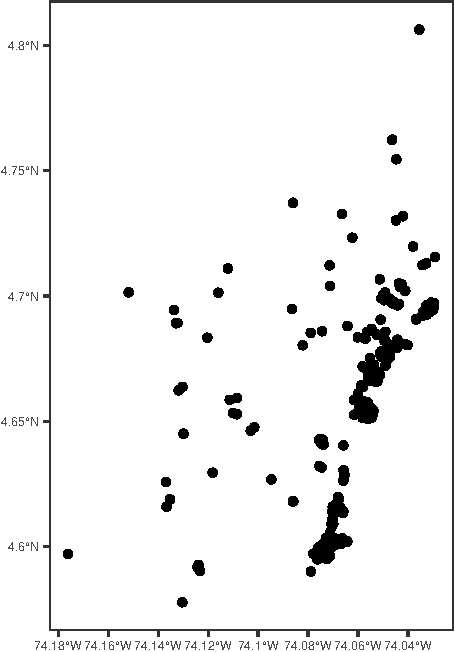
\includegraphics[scale=0.6]{figures/unnamed-chunk-1-1.pdf}
    \end{figure}
    \end{minipage}



\end{frame}
%----------------------------------------------------------------------%
\begin{frame}[fragile]
\frametitle{Visualizing Lines}



\begin{minipage}[t]{0.52\linewidth}
        \begin{scriptsize}

\begin{Shaded}
\begin{Highlighting}[]
\NormalTok{ciclovias\textless{}{-}}\KeywordTok{read\_sf}\NormalTok{(}\StringTok{"Ciclovia/Ciclovia.shp"}\NormalTok{)}
\KeywordTok{ggplot}\NormalTok{()}\OperatorTok{+}
\StringTok{  }\KeywordTok{geom\_sf}\NormalTok{(}\DataTypeTok{data=}\NormalTok{ciclovias) }\OperatorTok{+}
\StringTok{  }\KeywordTok{theme\_bw}\NormalTok{() }\OperatorTok{+}
\StringTok{  }\KeywordTok{theme}\NormalTok{(}\DataTypeTok{axis.title =}\KeywordTok{element\_blank}\NormalTok{(),}
        \DataTypeTok{panel.grid.major =} \KeywordTok{element\_blank}\NormalTok{(),}
        \DataTypeTok{panel.grid.minor =} \KeywordTok{element\_blank}\NormalTok{(),}
        \DataTypeTok{axis.text =} \KeywordTok{element\_text}\NormalTok{(}\DataTypeTok{size=}\DecValTok{6}\NormalTok{))}
\end{Highlighting}
\end{Shaded}
   \end{scriptsize}
    \end{minipage}
    \hfill
    \begin{minipage}[t]{0.43\linewidth}%
        \begin{figure}[H] \centering
            \captionsetup{justification=centering}  

            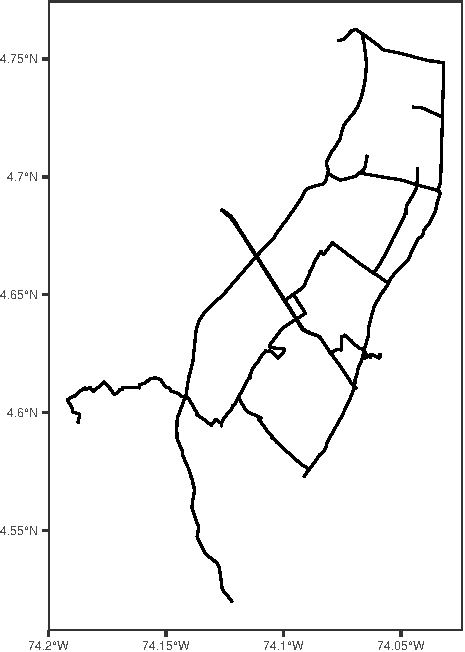
\includegraphics[scale=0.6]{figures/unnamed-chunk-2-1.pdf}
 \end{figure}
    \end{minipage}

\end{frame}
%----------------------------------------------------------------------%
\begin{frame}[fragile]
\frametitle{Visualizing  Polygons}


\begin{minipage}[t]{0.52\linewidth}
        \begin{scriptsize}

\begin{Shaded}
\begin{Highlighting}[]
\NormalTok{upla\textless{}{-}}\KeywordTok{read\_sf}\NormalTok{(}\StringTok{"upla/UPla.shp"}\NormalTok{)}

\KeywordTok{ggplot}\NormalTok{()}\OperatorTok{+}
\StringTok{  }\KeywordTok{geom\_sf}\NormalTok{(}\DataTypeTok{data=}\NormalTok{upla, }\KeywordTok{aes}\NormalTok{(}\DataTypeTok{fill =}\NormalTok{ UPlArea)) }\OperatorTok{+}
\StringTok{  }\KeywordTok{theme\_bw}\NormalTok{() }\OperatorTok{+}
\StringTok{  }\KeywordTok{theme}\NormalTok{(}\DataTypeTok{axis.title =}\KeywordTok{element\_blank}\NormalTok{(),}
        \DataTypeTok{panel.grid.major =} \KeywordTok{element\_blank}\NormalTok{(),}
        \DataTypeTok{panel.grid.minor =} \KeywordTok{element\_blank}\NormalTok{(),}
        \DataTypeTok{axis.text =} \KeywordTok{element\_text}\NormalTok{(}\DataTypeTok{size=}\DecValTok{6}\NormalTok{))}
\end{Highlighting}
\end{Shaded}
  \end{scriptsize}
    \end{minipage}
    \hfill
    \begin{minipage}[t]{0.43\linewidth}%
        \begin{figure}[H] \centering
            \captionsetup{justification=centering}

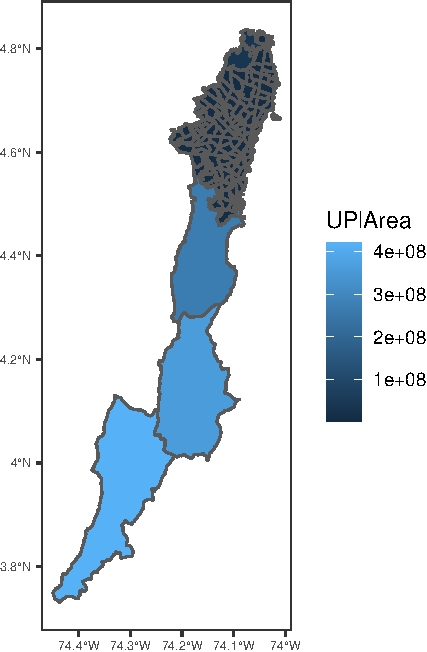
\includegraphics[scale=0.6]{figures/unnamed-chunk-2-2.pdf}
 \end{figure}
    \end{minipage}
\end{frame}
%----------------------------------------------------------------------%
\begin{frame}[fragile]
\frametitle{Visualizing Points, Lines, and Polygons}


\begin{minipage}[t]{0.52\linewidth}
        \begin{scriptsize}
\begin{Shaded}
\begin{Highlighting}[]
\KeywordTok{ggplot}\NormalTok{()}\OperatorTok{+}
\StringTok{  }\KeywordTok{geom\_sf}\NormalTok{(}\DataTypeTok{data=}\NormalTok{upla }
\OperatorTok{\%\textgreater{}\%}\StringTok{ }\KeywordTok{filter}\NormalTok{(}\KeywordTok{grepl}\NormalTok{(}\StringTok{"RIO"}\NormalTok{,UPlNombre)}\OperatorTok{==}\OtherTok{FALSE}\NormalTok{), }
\DataTypeTok{fill =} \OtherTok{NA}\NormalTok{) }\OperatorTok{+}
\StringTok{  }\KeywordTok{geom\_sf}\NormalTok{(}\DataTypeTok{data=}\NormalTok{ciclovias, }\DataTypeTok{col=}\StringTok{"red"}\NormalTok{) }\OperatorTok{+}
\StringTok{  }\KeywordTok{geom\_sf}\NormalTok{(}\DataTypeTok{data=}\NormalTok{bars) }\OperatorTok{+}
\StringTok{  }\KeywordTok{theme\_bw}\NormalTok{() }\OperatorTok{+}
\StringTok{  }\KeywordTok{theme}\NormalTok{(}\DataTypeTok{axis.title =}\KeywordTok{element\_blank}\NormalTok{(),}
        \DataTypeTok{panel.grid.major =} \KeywordTok{element\_blank}\NormalTok{(),}
        \DataTypeTok{panel.grid.minor =} \KeywordTok{element\_blank}\NormalTok{(),}
        \DataTypeTok{axis.text =} \KeywordTok{element\_text}\NormalTok{(}\DataTypeTok{size=}\DecValTok{6}\NormalTok{))}
\end{Highlighting}
\end{Shaded}
  \end{scriptsize}
    \end{minipage}
    \hfill
    \begin{minipage}[t]{0.43\linewidth}%
       \medskip
        \begin{figure}[H] \centering
            \captionsetup{justification=centering}
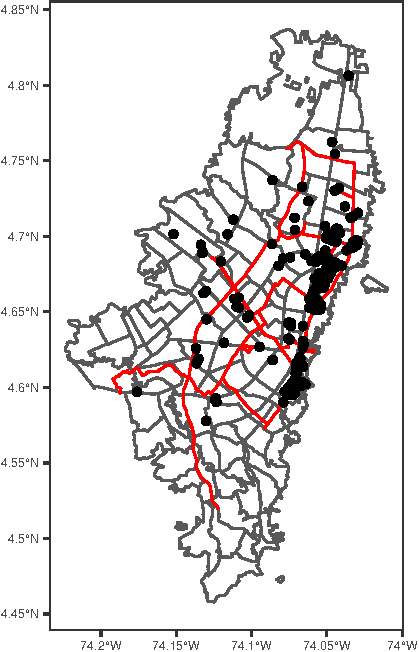
\includegraphics[scale=0.6]{figures/unnamed-chunk-3-1.pdf}

 \end{figure}
    \end{minipage}
\end{frame}

%----------------------------------------------------------------------%
\subsection{Creating Spatial Objects}
%----------------------------------------------------------------------%
\begin{frame}[fragile]
\frametitle{Creating Spatial Objects}

\begin{scriptsize}
\begin{Shaded}
\begin{Highlighting}[]
\NormalTok{db\textless{}{-}}\KeywordTok{data.frame}\NormalTok{(}\DataTypeTok{place=}\KeywordTok{c}\NormalTok{(}\StringTok{"Uniandes"}\NormalTok{,}\StringTok{"Banco de La Republica"}\NormalTok{),}
        \DataTypeTok{lat=}\KeywordTok{c}\NormalTok{(}\FloatTok{4.601590}\NormalTok{,}\FloatTok{4.602151}\NormalTok{), }
        \DataTypeTok{long=}\KeywordTok{c}\NormalTok{(}\OperatorTok{{-}}\FloatTok{74.066391}\NormalTok{,}\OperatorTok{{-}}\FloatTok{74.072350}\NormalTok{), }
        \DataTypeTok{nudge\_y=}\KeywordTok{c}\NormalTok{(}\OperatorTok{{-}}\FloatTok{0.001}\NormalTok{,}\FloatTok{0.001}\NormalTok{))}
\NormalTok{db\textless{}{-}db }\OperatorTok{\%\textgreater{}\%}\StringTok{ }\KeywordTok{mutate}\NormalTok{(}\DataTypeTok{latp=}\NormalTok{lat,}\DataTypeTok{longp=}\NormalTok{long)}
\NormalTok{db\textless{}{-}}\KeywordTok{st\_as\_sf}\NormalTok{(db,}\DataTypeTok{coords=}\KeywordTok{c}\NormalTok{(}\StringTok{\textquotesingle{}longp\textquotesingle{}}\NormalTok{,}\StringTok{\textquotesingle{}latp\textquotesingle{}}\NormalTok{),}\DataTypeTok{crs=}\DecValTok{4326}\NormalTok{)}
\end{Highlighting}
\end{Shaded}
\end{scriptsize}
\begin{minipage}[t]{0.52\linewidth}
        \begin{tiny}
        \begin{Shaded}
\begin{Highlighting}[]
\KeywordTok{ggplot}\NormalTok{()}\OperatorTok{+}
\StringTok{  }\KeywordTok{geom\_sf}\NormalTok{(}\DataTypeTok{data=}\NormalTok{upla }
    \OperatorTok{\%\textgreater{}\%}\StringTok{ }\KeywordTok{filter}\NormalTok{(UPlNombre}
    \OperatorTok{\%in\%}\KeywordTok{c}\NormalTok{(}\StringTok{"LA CANDELARIA"}\NormalTok{,}\StringTok{"LAS NIEVES"}\NormalTok{)), }\DataTypeTok{fill =} \OtherTok{NA}\NormalTok{) }\OperatorTok{+}
\StringTok{  }\KeywordTok{geom\_sf}\NormalTok{(}\DataTypeTok{data=}\NormalTok{db, }\DataTypeTok{col=}\StringTok{"red"}\NormalTok{) }\OperatorTok{+}
\StringTok{  }\KeywordTok{geom\_label}\NormalTok{(}\DataTypeTok{data =}\NormalTok{ db, }\KeywordTok{aes}\NormalTok{(}\DataTypeTok{x =}\NormalTok{ long, }\DataTypeTok{y =}\NormalTok{ lat, }
                \DataTypeTok{label =}\NormalTok{ place), }
        \DataTypeTok{size =} \DecValTok{3}\NormalTok{, }\DataTypeTok{col =} \StringTok{"black"}\NormalTok{, }\DataTypeTok{fontface =} \StringTok{"bold"}\NormalTok{, }
        \DataTypeTok{nudge\_y =}\NormalTok{db}\OperatorTok{$}\NormalTok{nudge\_y) }\OperatorTok{+}
\StringTok{  }\KeywordTok{theme\_bw}\NormalTok{() }\OperatorTok{+}
\StringTok{  }\KeywordTok{theme}\NormalTok{(}\DataTypeTok{axis.title =}\KeywordTok{element\_blank}\NormalTok{(),}
        \DataTypeTok{panel.grid.major =} \KeywordTok{element\_blank}\NormalTok{(),}
        \DataTypeTok{panel.grid.minor =} \KeywordTok{element\_blank}\NormalTok{(),}
        \DataTypeTok{axis.text =} \KeywordTok{element\_text}\NormalTok{(}\DataTypeTok{size=}\DecValTok{6}\NormalTok{))}
\end{Highlighting}
\end{Shaded}
  \end{tiny}
    \end{minipage}
    \hfill
    \begin{minipage}[t]{0.43\linewidth}%
       \medskip
        \begin{figure}[H] \centering
            \captionsetup{justification=centering}
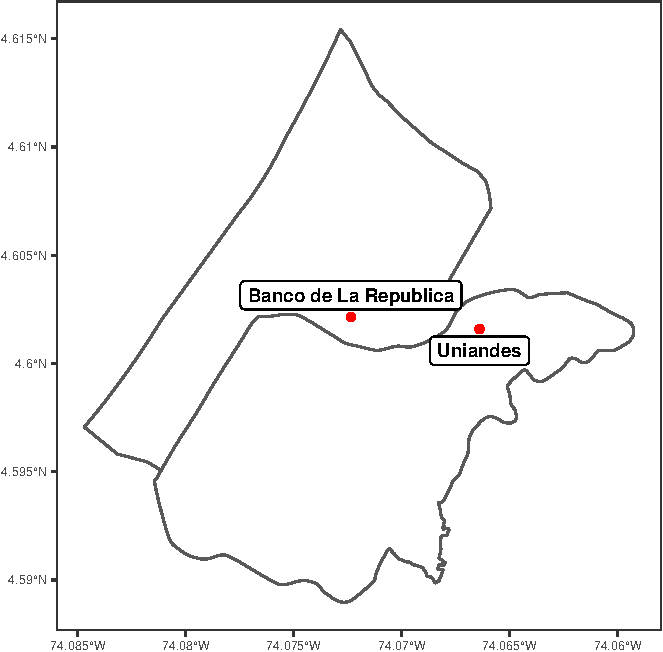
\includegraphics[scale=0.43]{figures/unnamed-chunk-4-1.pdf}

    \end{figure}
    \end{minipage}

\end{frame}

%----------------------------------------------------------------------%
\subsection{Measuring Distances}
%----------------------------------------------------------------------%
\begin{frame}[fragile]
\frametitle{Measuring Distances}

\begin{Shaded}
\begin{Highlighting}[]
\KeywordTok{st\_distance}\NormalTok{(db)}
\end{Highlighting}
\end{Shaded}
\begin{scriptsize}
\begin{verbatim}
## Units: [m]
##          [,1]     [,2]
## [1,]   0.0000 664.1323
## [2,] 664.1323   0.0000
\end{verbatim}
\end{scriptsize}

\begin{figure}[H] \centering
  \centering
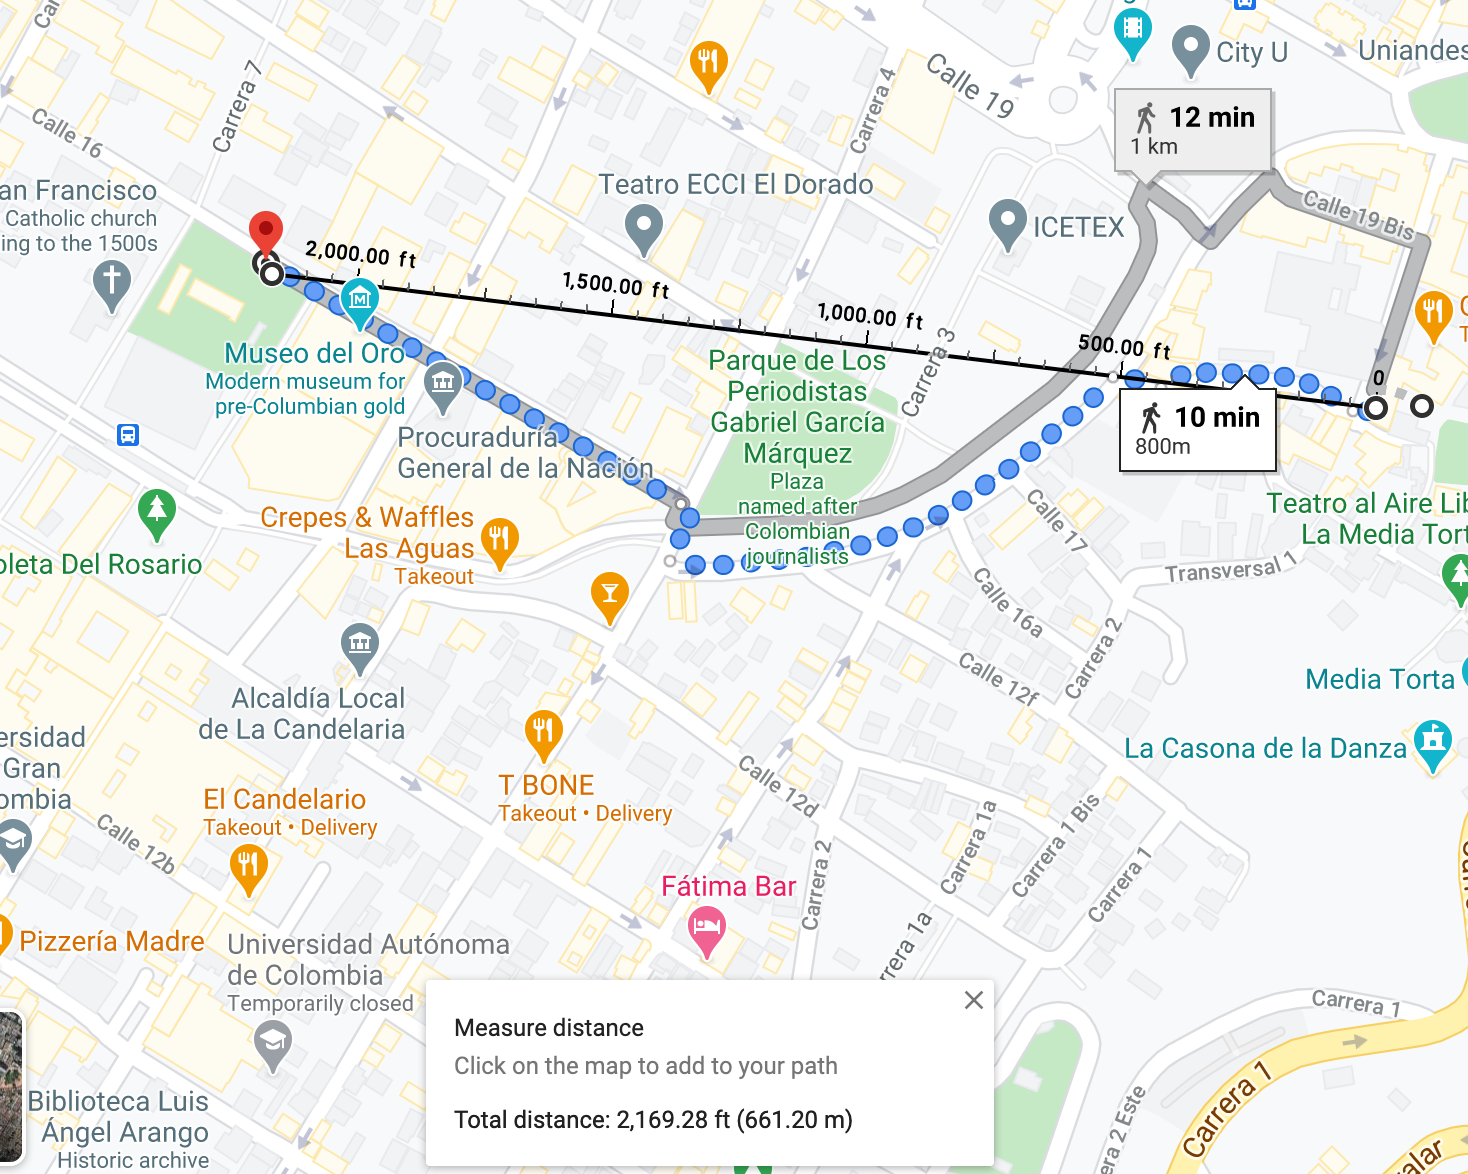
\includegraphics[scale=0.25]{figures/distance_google_maps}
  \\
  \end{figure}



\end{frame}
%----------------------------------------------------------------------%
\begin{frame}[fragile]
\frametitle{Measuring Distances}

\begin{scriptsize}
\begin{Shaded}
\begin{Highlighting}[]
\KeywordTok{st\_distance}\NormalTok{(db,ciclovias)}
\ErrorTok{Error in st_distance(db, ciclovias) : st_crs(x) == st_crs(y) is not TRUE}
\KeywordTok{st\_crs}\NormalTok{(ciclovias)}
\end{Highlighting}
\end{Shaded}
\end{scriptsize}
\begin{tiny}
\begin{verbatim}
## Coordinate Reference System:
##   User input: 3857 
##   wkt:
## PROJCS["WGS 84 / Pseudo-Mercator",
##     GEOGCS["WGS 84",
##         DATUM["WGS_1984",
##             SPHEROID["WGS 84",6378137,298.257223563,
##                 AUTHORITY["EPSG","7030"]],
##             AUTHORITY["EPSG","6326"]],
##         PRIMEM["Greenwich",0,
##             AUTHORITY["EPSG","8901"]],
##         UNIT["degree",0.0174532925199433,
##             AUTHORITY["EPSG","9122"]],
##         AUTHORITY["EPSG","4326"]],
##     PROJECTION["Mercator_1SP"],
##     PARAMETER["central_meridian",0],
##     PARAMETER["scale_factor",1],
##     PARAMETER["false_easting",0],
##     PARAMETER["false_northing",0],
##     UNIT["metre",1,
##         AUTHORITY["EPSG","9001"]],
##     AXIS["X",EAST],
##     AXIS["Y",NORTH],
##     EXTENSION["PROJ4","+proj=merc +a=6378137 +b=6378137 +lat_ts=0.0 +lon_0=0.0 +x_0=0.0 +y_0=0 +k=1.0 +units=m +nadgrids=@null +wktext +no_defs"],
##     AUTHORITY["EPSG","3857"]]
\end{verbatim}
\end{tiny}
\end{frame}
%----------------------------------------------------------------------%
\begin{frame}[fragile]
\frametitle{Measuring Distances}

\begin{scriptsize}
\begin{Shaded}
\begin{Highlighting}[]
\NormalTok{ciclovias\textless{}{-}}\KeywordTok{st\_transform}\NormalTok{(ciclovias, }\DecValTok{4686}\NormalTok{)}
\KeywordTok{st\_crs}\NormalTok{(ciclovias)}
\end{Highlighting}
\end{Shaded}
\begin{tiny}
\begin{verbatim}
## Coordinate Reference System:
##   User input: EPSG:4686 
##   wkt:
## GEOGCS["MAGNA-SIRGAS",
##     DATUM["Marco_Geocentrico_Nacional_de_Referencia",
##         SPHEROID["GRS 1980",6378137,298.257222101,
##             AUTHORITY["EPSG","7019"]],
##         TOWGS84[0,0,0,0,0,0,0],
##         AUTHORITY["EPSG","6686"]],
##     PRIMEM["Greenwich",0,
##         AUTHORITY["EPSG","8901"]],
##     UNIT["degree",0.0174532925199433,
##         AUTHORITY["EPSG","9122"]],
##     AUTHORITY["EPSG","4686"]]
\end{verbatim}
\end{tiny}
\begin{Shaded}
\begin{Highlighting}[]
\NormalTok{db\textless{}{-}}\KeywordTok{st\_transform}\NormalTok{(db, }\DecValTok{4326}\NormalTok{)}
\KeywordTok{st\_distance}\NormalTok{(db,ciclovias)}
\end{Highlighting}
\end{Shaded}

\begin{verbatim}
## Units: [m]
##          [,1]     [,2]     [,3]     [,4]     [,5]     [,6]     [,7]     [,8]
## [1,] 9514.617 10789.90 6035.283 12855.90 6025.017 8311.922 4579.450 741.6047
## [2,] 9221.998 10686.39 6143.960 13004.84 5871.073 7656.183 4014.993 116.5939
##           [,9]    [,10]    [,11]    [,12]    [,13]    [,14]
## [1,] 1002.8751 6255.692 2385.125 8402.580 8669.030 3788.265
## [2,]  981.1991 5839.565 2425.508 7738.774 8048.108 3436.819
\end{verbatim}
\end{scriptsize}
\end{frame}
%----------------------------------------------------------------------%
\begin{frame}[fragile]
\frametitle{Measuring Distances}


\begin{minipage}[t]{0.52\linewidth}
        \begin{scriptsize}
\begin{Shaded}
\begin{Highlighting}[]
\NormalTok{ciclovias\_sp\textless{}{-}ciclovias[}\DecValTok{8}\NormalTok{,]}

\KeywordTok{ggplot}\NormalTok{()}\OperatorTok{+}
\StringTok{  }\KeywordTok{geom\_sf}\NormalTok{(}\DataTypeTok{data=}\NormalTok{ciclovias[}\DecValTok{8}\NormalTok{,], }\DataTypeTok{fill =} \OtherTok{NA}\NormalTok{) }\OperatorTok{+}
\StringTok{  }\KeywordTok{geom\_sf}\NormalTok{(}\DataTypeTok{data=}\NormalTok{db, }\DataTypeTok{col=}\StringTok{"red"}\NormalTok{) }\OperatorTok{+}
\StringTok{  }\KeywordTok{theme\_bw}\NormalTok{() }\OperatorTok{+}
\StringTok{  }\KeywordTok{theme}\NormalTok{(}\DataTypeTok{axis.title =}\KeywordTok{element\_blank}\NormalTok{(),}
        \DataTypeTok{panel.grid.major =} \KeywordTok{element\_blank}\NormalTok{(),}
        \DataTypeTok{panel.grid.minor =} \KeywordTok{element\_blank}\NormalTok{(),}
        \DataTypeTok{axis.text =} \KeywordTok{element\_text}\NormalTok{(}\DataTypeTok{size=}\DecValTok{6}\NormalTok{))}
\end{Highlighting}
\end{Shaded}
  \end{scriptsize}
    \end{minipage}
    \hfill
    \begin{minipage}[t]{0.43\linewidth}%
       \medskip
        \begin{figure}[H] \centering
            \captionsetup{justification=centering}
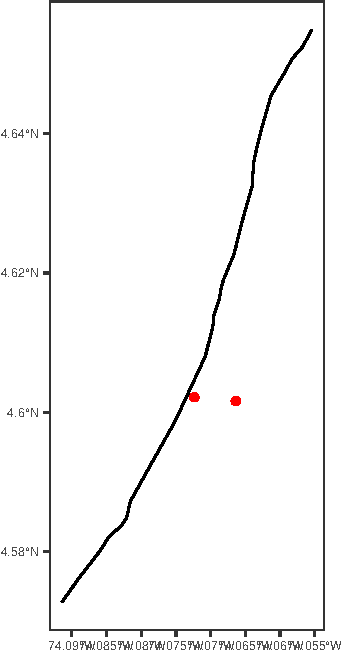
\includegraphics[scale=0.6]{figures/unnamed-chunk-7-1.pdf}

    \end{figure}
    \end{minipage}

\end{frame}

%----------------------------------------------------------------------%
\subsection{Weights Matrix in \texttt{R}}
%----------------------------------------------------------------------%
\begin{frame}[fragile]
\frametitle{Weights Matrix in \texttt{R}}


\begin{scriptsize}
\begin{Shaded}
\begin{Highlighting}[]
\KeywordTok{require}\NormalTok{(}\StringTok{"sf"}\NormalTok{)}
\KeywordTok{require}\NormalTok{(}\StringTok{"spdep"}\NormalTok{)}
\KeywordTok{require}\NormalTok{(}\StringTok{"dplyr"}\NormalTok{)}
\end{Highlighting}
\end{Shaded}

\begin{Shaded}
\begin{Highlighting}[]
\NormalTok{chi.poly\textless{}{-}}\KeywordTok{read\_sf}\NormalTok{(}\StringTok{"foreclosures/foreclosures.shp"}\NormalTok{)}
\KeywordTok{st\_crs}\NormalTok{(chi.poly) }\CommentTok{\#doesn't have a projection}
\end{Highlighting}
\end{Shaded}

\end{scriptsize}

\begin{verbatim}
## Coordinate Reference System: NA
\end{verbatim}

\begin{scriptsize}
\begin{Shaded}
\begin{Highlighting}[]
\KeywordTok{st\_crs}\NormalTok{(chi.poly)\textless{}{-}}\DecValTok{4326} \CommentTok{\#WGS84 set it in the map}
\end{Highlighting}
\end{Shaded}
\end{scriptsize}

\end{frame}

%----------------------------------------------------------------------%
\begin{frame}[fragile]
\frametitle{Weights Matrix in \texttt{R}}

\begin{scriptsize}

\begin{Shaded}
\begin{Highlighting}[]
\NormalTok{chi.poly\textless{}{-}}\KeywordTok{st\_transform}\NormalTok{(chi.poly,}\DecValTok{26916}\NormalTok{) }\CommentTok{\#reproject planarly}
\CommentTok{\#NAD83 UTM Zone 16N}
\KeywordTok{st\_crs}\NormalTok{(chi.poly)}
\end{Highlighting}
\end{Shaded}
\end{scriptsize}
\begin{tiny}
\begin{verbatim}
## Coordinate Reference System:
##   User input: EPSG:26916 
##   wkt:
## PROJCS["NAD83 / UTM zone 16N",
##     GEOGCS["NAD83",
##         DATUM["North_American_Datum_1983",
##             SPHEROID["GRS 1980",6378137,298.257222101,
##                 AUTHORITY["EPSG","7019"]],
##             TOWGS84[0,0,0,0,0,0,0],
##             AUTHORITY["EPSG","6269"]],
##         PRIMEM["Greenwich",0,
##             AUTHORITY["EPSG","8901"]],
##         UNIT["degree",0.0174532925199433,
##             AUTHORITY["EPSG","9122"]],
##         AUTHORITY["EPSG","4269"]],
##     PROJECTION["Transverse_Mercator"],
##     PARAMETER["latitude_of_origin",0],
##     PARAMETER["central_meridian",-87],
##     PARAMETER["scale_factor",0.9996],
##     PARAMETER["false_easting",500000],
##     PARAMETER["false_northing",0],
##     UNIT["metre",1,
##         AUTHORITY["EPSG","9001"]],
##     AXIS["Easting",EAST],
##     AXIS["Northing",NORTH],
##     AUTHORITY["EPSG","26916"]]
\end{verbatim}

\end{tiny}
\end{frame}

%----------------------------------------------------------------------%
\begin{frame}[fragile]
\frametitle{Weights Matrix in \texttt{R}}

\begin{scriptsize}
\begin{Shaded}
\begin{Highlighting}[]
\KeywordTok{str}\NormalTok{(chi.poly)}
\end{Highlighting}
\end{Shaded}
\end{scriptsize}
\begin{tiny}


\begin{verbatim}
## tibble [897 x 17] (S3: sf/tbl_df/tbl/data.frame)
##  $ SP_ID     : chr [1:897] "1" "2" "3" "4" ...
##  $ fips      : chr [1:897] "17031010100" "17031010200" "17031010300" "17031010400" ...
##  $ est_fcs   : int [1:897] 43 129 55 21 64 56 107 43 7 51 ...
##  $ est_mtgs  : int [1:897] 904 2122 1151 574 1427 1241 1959 830 208 928 ...
##  $ est_fcs_rt: num [1:897] 4.76 6.08 4.78 3.66 4.48 4.51 5.46 5.18 3.37 5.5 ...
##  $ res_addr  : int [1:897] 2530 3947 3204 2306 5485 2994 3701 1694 443 1552 ...
##  $ est_90d_va: num [1:897] 12.61 12.36 10.46 5.03 8.44 ...
##  $ bls_unemp : num [1:897] 8.16 8.16 8.16 8.16 8.16 8.16 8.16 8.16 8.16 8.16 ...
##  $ county    : chr [1:897] "Cook County" "Cook County" "Cook County" "Cook County" ...
##  $ fips_num  : num [1:897] 1.7e+10 1.7e+10 1.7e+10 1.7e+10 1.7e+10 ...
##  $ totpop    : int [1:897] 5391 10706 6649 5325 10944 7178 10799 5403 1089 3634 ...
##  $ tothu     : int [1:897] 2557 3981 3281 2464 5843 3136 3875 1768 453 1555 ...
##  $ huage     : int [1:897] 61 53 56 60 54 58 48 57 61 48 ...
##  $ oomedval  : int [1:897] 169900 147000 119800 151500 143600 145900 153400 170500 215900 114700 ...
##  $ property  : num [1:897] 646 914 478 509 641 612 678 332 147 351 ...
##  $ violent   : num [1:897] 433 421 235 159 240 266 272 146 78 84 ...
##  $ geometry  :sfc_POLYGON of length 897; first list element: List of 1
##   ..$ : num [1:15, 1:2] 443923 444329 444814 444839 444935 ...
##   ..- attr(*, "class")= chr [1:3] "XY" "POLYGON" "sfg"
##  - attr(*, "sf_column")= chr "geometry"
##  - attr(*, "agr")= Factor w/ 3 levels "constant","aggregate",..: NA NA NA NA NA NA NA NA NA NA ...
##   ..- attr(*, "names")= chr [1:16] "SP_ID" "fips" "est_fcs" "est_mtgs" ...
\end{verbatim}
\end{tiny}

\end{frame}


%----------------------------------------------------------------------%
\begin{frame}[fragile]
\frametitle{Weights Matrix in \texttt{R}}

\begin{scriptsize}
\begin{Shaded}
\begin{Highlighting}[]
\KeywordTok{plot}\NormalTok{(chi.poly[}\StringTok{\textquotesingle{}violent\textquotesingle{}}\NormalTok{])}
\end{Highlighting}
\end{Shaded}
\end{scriptsize}



  \begin{figure}[H] \centering
    \captionsetup{justification=centering}
    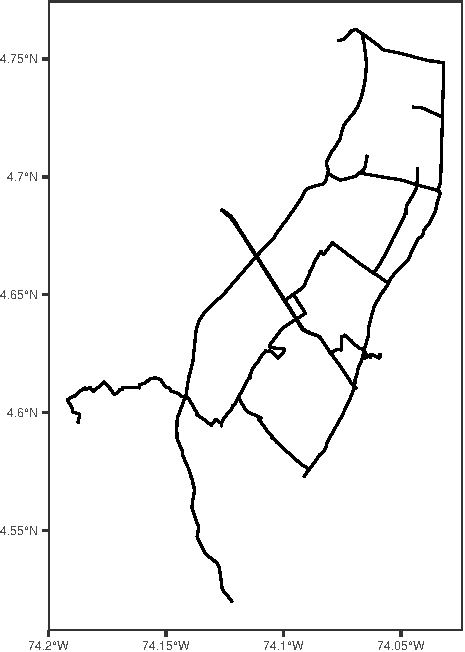
\includegraphics[scale=0.5]{figures/unnamed-chunk-2-1.pdf}
   \end{figure}



\end{frame}


%----------------------------------------------------------------------%
\begin{frame}[fragile]
\frametitle{Weights Matrix in \texttt{R}}


\begin{scriptsize}
\begin{Shaded}
\begin{Highlighting}[]
\NormalTok{list.queen\textless{}{-}}\KeywordTok{poly2nb}\NormalTok{(chi.poly, }\DataTypeTok{queen=}\OtherTok{TRUE}\NormalTok{)}
\NormalTok{W\textless{}{-}}\KeywordTok{nb2listw}\NormalTok{(list.queen, }\DataTypeTok{style=}\StringTok{"W"}\NormalTok{, }\DataTypeTok{zero.policy=}\OtherTok{TRUE}\NormalTok{)}
\NormalTok{W}
\end{Highlighting}
\end{Shaded}
\end{scriptsize}

\begin{tiny}
\begin{verbatim}
## Characteristics of weights list object:
## Neighbour list object:
## Number of regions: 897 
## Number of nonzero links: 6140 
## Percentage nonzero weights: 0.7631036 
## Average number of links: 6.845039 
## 
## Weights style: W 
## Weights constants summary:
##     n     nn  S0       S1       S2
## W 897 804609 897 274.4893 3640.864
\end{verbatim}

\end{tiny}

\end{frame}

%----------------------------------------------------------------------%
\begin{frame}[fragile]
\frametitle{Weights Matrix in \texttt{R}}


\begin{scriptsize}
\begin{Shaded}
\begin{Highlighting}[]
\KeywordTok{plot}\NormalTok{(W,}\KeywordTok{st\_geometry}\NormalTok{(}\KeywordTok{st\_centroid}\NormalTok{(chi.poly)))}
\end{Highlighting}
\end{Shaded}
\end{scriptsize}


 \begin{figure}[H] \centering
    \captionsetup{justification=centering}
    
\includegraphics[scale=0.7]{figures/neighbors_plot-1.pdf}
   \end{figure}


\end{frame}

%----------------------------------------------------------------------%
\begin{frame}[fragile]
\frametitle{Weights Matrix in \texttt{R}}


\begin{scriptsize}
\begin{Shaded}
\begin{Highlighting}[]
\NormalTok{coords \textless{}{-}}\StringTok{ }\KeywordTok{st\_centroid}\NormalTok{(}\KeywordTok{st\_geometry}\NormalTok{(chi.poly), }\DataTypeTok{of\_largest\_polygon=}\OtherTok{TRUE}\NormalTok{)}
\NormalTok{W\_dist\textless{}{-}}\KeywordTok{dnearneigh}\NormalTok{(coords,}\DecValTok{0}\NormalTok{,}\DecValTok{1000}\NormalTok{)}
\NormalTok{W\_dist}
\end{Highlighting}
\end{Shaded}
\end{scriptsize}
\begin{tiny}
\begin{verbatim}
## Neighbour list object:
## Number of regions: 897 
## Number of nonzero links: 5448 
## Percentage nonzero weights: 0.6770991 
## Average number of links: 6.073579 
## 55 regions with no links:
## 141 142 143 145 153 154 155 158 462 631 637 638 642 643 644 645 655 656 657 658 659 758 759 769 820 821 822 823 824 855 856 857 861 862 864 865 866 867 868 870 871 872 873 876 877 880 885 886 887 888 889 890 892 896 897
\end{verbatim}

\end{tiny}


\begin{scriptsize}
\begin{Shaded}
\begin{Highlighting}[]
\KeywordTok{plot}\NormalTok{(W\_dist, coords)}
\end{Highlighting}
\end{Shaded}

\end{scriptsize}


 \begin{figure}[H] \centering
    \captionsetup{justification=centering}
    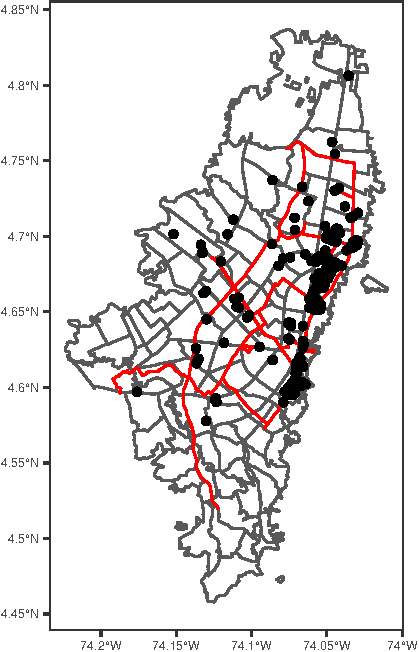
\includegraphics[scale=0.7]{figures/unnamed-chunk-3-1.pdf}
   \end{figure}



\end{frame}

%----------------------------------------------------------------------%
\begin{frame}[fragile]
\frametitle{Weights Matrix in \texttt{R}}

\begin{scriptsize}
\begin{Shaded}
\begin{Highlighting}[]
\NormalTok{W\_dist\textless{}{-}}\KeywordTok{dnearneigh}\NormalTok{(coords,}\DecValTok{0}\NormalTok{,}\DecValTok{4300}\NormalTok{)}
\NormalTok{W\_dist}
\end{Highlighting}
\end{Shaded}
\end{scriptsize}

\begin{tiny}
\begin{verbatim}
## Neighbour list object:
## Number of regions: 897 
## Number of nonzero links: 87988 
## Percentage nonzero weights: 10.9355 
## Average number of links: 98.09142
\end{verbatim}
\end{tiny}

\begin{scriptsize}
\begin{Shaded}
\begin{Highlighting}[]
\KeywordTok{plot}\NormalTok{(W\_dist, coords)}
\end{Highlighting}
\end{Shaded}
\end{scriptsize}


 \begin{figure}[H] \centering
    \captionsetup{justification=centering}
    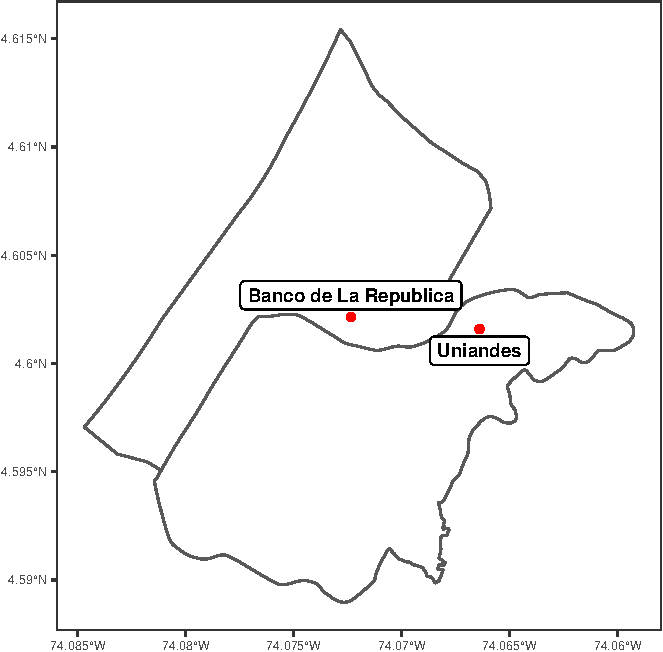
\includegraphics[scale=0.7]{figures/unnamed-chunk-4-1.pdf}
   \end{figure}



\end{frame}




%----------------------------------------------------------------------%
%----------------------------------------------------------------------%
\end{document}
%----------------------------------------------------------------------%
%----------------------------------------------------------------------%

